%%%% Шаблон ВКР <<SPbPU-student-thesis-template>>  %%%%
%%
%%   Создан на основе глубокой переработки шаблона российских кандидатских и докторских диссертаций [1]. 
%%   
%%   Полный список различий может быть получен командами git.
%%   Лист авторов-составителей расположен в README.md файле.
%%   Подробные инструкции по использованию в [1,2].
%%   
%%   Рекомендуем установить TeX Live + TeXstudio
%%   <<Стандартная>> компиляция 2-3 РАЗА с помощью pdflatex + biber (для библиографии)     
%%  
%%%% Student thesis template <<SPbPU-student-thesis-template>> %%%%
%%
%%   Created on the basis of deepl modifification of the Russian candidate and doctorate thesis template [1]. 
%%   
%%   Full list of differences can be achieved by git commands.
%%   List of template authors can be seen in the README.md file.
%%   Detailed instructions of usage, see, please in [1,2].
%%     
%%   [1] github.com/AndreyAkinshin/Russian-Phd-LaTeX-Dissertation-Template 
%%   [2] Author_guide_SPBPU-student-thesis-template.pdf
%%   
%%   It is recommended to install TeX Live + TeXstudio   
%%   Default compilation 2-3 TIMES with pdflatex + biber (for the bibliography)
%%  
\input{template_settings/ch_preamble} % лучше не редактировать / please, keep unmodified


%%%% Настройки автора / Author settings
%% 
\input{my_folder/my_settings} % добавляем свои команды / update your commands


\begin{document} % начало документа

%%% Внесите свои данные - Input your data
%%
%%
\newcommand{\Author}{О.Ю.\,Григорьев} % И.О. Фамилия автора
\newcommand{\AuthorFull}{Григорьев Олег Юрьевич} % Фамилия Имя Отчество автора
\newcommand{\AuthorFullDat}{Григорьеву Олегу Юрьевичу} % Фамилия Имя Отчество автора в дательном падеже (Кому? Студенту...)
\newcommand{\AuthorFullVin}{Григорьева Олега Юрьевича} % в винительном падеже (Кого? что?  Програмиста ...)
\newcommand{\AuthorPhone}{+7-911-088-88-48} % номер телефорна автора для оперативной связи
\newcommand{\Supervisor}{В.Г.\,Пак} % И. О. Фамилия научного руководителя
\newcommand{\SupervisorFull}{Пак Вадим Геннадьевич} % Фамилия Имя Отчество научного руководителя
\newcommand{\SupervisorVin}{В.Г.\,Пака} % И. О. Фамилия научного руководителя  в винительном падеже (Кого? что? Руководителя ...)
\newcommand{\SupervisorJob}{доцент ВШИСиСТ} %
\newcommand{\SupervisorJobVin}{доцента ВШиСТ} % в винительном падеже (Кого? что?  Програмиста ...)
\newcommand{\SupervisorDegree}{к.ф.-м.н.} %
\newcommand{\SupervisorTitle}{звание} %
%%
%%
%Руководитель, утверждающий задание
\newcommand{\Head}{В.Г.\,Пак} % И. О. Фамилия руководителя подразделения (руководителя ОП)
\newcommand{\HeadDegree}{Руководитель ОП}% Только должность:
%Руководитель %ОП 
%Заведующий % кафедрой
%Директор % Высшей школы
%Зам. директора
\newcommand{\HeadDep}{} % заменить на краткую аббревиатуру подразделения или оставить пустым, если утверждает руководитель ОП

%%% Руководитель, принимающий заявление
\newcommand{\HeadAp}{И.О.\,Фамилия} % И. О. Фамилия руководителя подразделения (руководителя ОП)
\newcommand{\HeadApDegree}{Должность руководителя}% Только должность:   
%Руководитель ОП 
%Заведующий кафедрой
%Директор Высшей школы
\newcommand{\HeadApDep}{O} % заменить на краткую аббревиатуру подразделения или оставить пустым, если утверждает руководитель ОП
%%% Консультант по нормоконтролю
\newcommand{\ConsultantNorm}{Ю.Д.\,Заковряшин} % И. О. Фамилия консультанта по нормоконтролю. ТОЛЬКО из числа ППС!
\newcommand{\ConsultantNormDegree}{Старший преподаватель ВШИСиСТ} %
%%% Первый консультант
\newcommand{\ConsultantExtraFull}{Заковряшин Юрий Дмитриевич} % Фамилия Имя Отчетство дополнительного консультанта
\newcommand{\ConsultantExtra}{И.О.\,Фамилия} % И. О. Фамилия дополнительного консультанта 
\newcommand{\ConsultantExtraDegree}{должность, степень} % 
\newcommand{\ConsultantExtraVin}{И.О.\,Фамилию} % И. О. Фамилия дополнительного консультанта в винительном падеже (Кого? что? Руководителя ...)
\newcommand{\ConsultantExtraDegreeVin}{должность, степень} %  в винительном падеже (Кого? что? Руководителя ...)
%%% Второй консультант
\newcommand{\ConsultantExtraTwoFull}{Фамилия Имя Отчетство} % Фамилия Имя Отчетство дополнительного консультанта
\newcommand{\ConsultantExtraTwo}{И.О.\,Фамилия} % И. О. Фамилия дополнительного консультанта
\newcommand{\ConsultantExtraTwoDegree}{должность, степень} %
\newcommand{\ConsultantExtraTwoVin}{И.О.\,Фамилию} % И. О. Фамилия дополнительного консультанта в винительном падеже (Кого? что? Руководителя ...)
\newcommand{\ConsultantExtraTwoDegreeVin}{должность, степень} %  в винительном падеже (Кого? что? Руководителя ...)
\newcommand{\Reviewer}{И.О.\,Фамилия} % И. О. Фамилия резензента. Обязателен только для магистров.
\newcommand{\ReviewerDegree}{должность, степень} % 
%%
%%
\renewcommand{\thesisTitle}{Исследование применения технологии обучения с подкреплением в управлении мультиагентной системой в игровой среде}
%\newcommand{\thesisDegree}{бакалавра}% магистра или специалиста%
\newcommand{\thesisDegree}{магистерская диссертация}% дипломный проект, дипломная работа, магистерская диссертация %c 2020
\newcommand{\thesisTitleEn}{Investigation of the Application of Reinforcement Learning to Managing Multi-Agent systems in Gaming Environment} %2020
\newcommand{\thesisDeadline}{05.2020}
\newcommand{\thesisStartDate}{03.02.2020}
\newcommand{\thesisYear}{2020}
%%
%%
\newcommand{\group}{в3540203/80277} % заменить вместо N номер группы
\newcommand{\thesisSpecialtyCode}{02.04.03}% код направления подготовки
\newcommand{\thesisSpecialtyTitle}{\mbox{Математическое} \mbox{обеспечение} и \mbox{администрирование} \mbox{информационных} \mbox{систем}} % наименование направления/специальности
\newcommand{\thesisOPPostfix}{02} % последние цифры кода образовательной программы (после <<_>>)
\newcommand{\thesisOPTitle}{\mbox{Проектирование} и \mbox{разработка} \mbox{информационных} \mbox{систем}}% наименование образовательной программы
%%
%%
\newcommand{\institute}{
%Название института
Институт компьютерных наук и технологий
%Гуманитарный институт
%Инженерно-строительный институт
%Институт биомедицинских систем и технологий
%Институт металлургии, машиностроения и транспорта
%Институт передовых производственных технологий
%Институт прикладной математики и механики
%Институт физики, нанотехнологий и телекоммуникаций
%Институт физической культуры, спорта и туризма
%Институт энергетики и транспортных систем
%Институт промышленного менеджмента, экономики и торговли
}%
%%
%%




%%% Задание ключевых слов и аннотации
%%
%%
%% Ключевых слов от 3 до 5 слов или словосочетаний в именительном падеже именительном падеже множественного числа (или в единственном числе, если нет другой формы) по правилам русского языка!!!
%%
%%
\newcommand{\keywordsRu}{Машинное обучение, обучение с подкреплением, глубокое обучение, мультиагентные системы} % ВВЕДИТЕ ключевые слова по-русски
%%
%%
\newcommand{\keywordsEn}{Machine Learning, Reinforcement Learning, Deep Learning, Multi-Agent Systems} % ВВЕДИТЕ ключевые слова по-английски
%%
%%
%% Реферат ОТ 1000 ДО 1500 знаков на русский или английский текст
%%
%Реферат должен содержать:
%- предмет, тему, цель ВКР;
%- метод или методологию проведения ВКР:
%- результаты ВКР:
%- область применения результатов ВКР;
%- выводы.

\newcommand{\abstractRu}{В данной работе исследована технология обучения с подкреплением, её применимость к мультиагентным системам, а именно применимость алгоритма мультиагентной глубокой детерминированной политики градиента (MADDPG). Изучено общение агентов между собой. Были предложены, реализованы и протестированы различные способы оптимизации обучения. Эксперименты производились в различных сценариях в двухмерной среде multiagent-particle-envs \cite{multiagent-particle-envs} от компании OpenAI.} % ВВЕДИТЕ текст аннотации по-русски
%%
%%
\newcommand{\abstractEn}{In this thesis Reinforcement Learning and its applicability to Multi-Agent systems were examined. Specifically, Multi-Agent Deep Deterministic Policy Gradient was reviewed. Communication between agents was researched. Different optimizing methods were suggested, implemented, and tested. Experiments were set up on different scenarios in 2D-environment  multiagent-particle-envs \cite{multiagent-particle-envs} by OpenAI.} % ВВЕДИТЕ текст аннотации по-английски


%%% РАЗДЕЛ ДЛЯ ОФОРМЛЕНИЯ ПРАКТИКИ
%Место прохождения практики
\newcommand{\PracticeType}{Отчет о прохождении %
	%стационарной производственной (технологической (проектно-технологической)) %
	такой-то % тип и вид ЗАМЕНИТЬ
	практики}

\newcommand{\Workplace}{СПбПУ, ИКНТ, ВШИСиСТ} % TODO Rename this variable

% Даты начала/окончания
\newcommand{\PracticeStartDate}{%
дд.мм.гггг%
%	22.06.2020
}%
\newcommand{\PracticeEndDate}{%
	дд.мм.гггг%
%	18.07.2020%
}%
%%

\newcommand{\School}{
%	Название высшей школы
	Высшая школа интеллектуальных систем и~суперкомпьютерных~технологий
}
\newcommand{\practiceTitle}{Тема практики}


%% ВНИМАНИЕ! Необходимо либо заменить текст аннотации (ключевых слов) на русском и английском, либо удалить там весь текст, иначе в свойства pdf-отчета по практике пойдет шаблонный текст.

%%% Не меняем дальнейшую часть - Do not modify the rest part
%%
%%
%%
%%
\ifnumequal{\value{docType}}{1}{% Если ВКР, то...
	\newcommand{\DocType}{Выпускная квалификационная работа}
	\newcommand{\pdfDocType}{\DocType~(\thesisDegree)} %задаём метаданные pdf файла
	\newcommand{\pdfTitle}{\thesisTitle}
}{% Иначе
	\newcommand{\DocType}{\PracticeType}
	\newcommand{\pdfDocType}{\DocType} %задаём метаданные pdf файла
	\newcommand{\pdfTitle}{\practiceTitle}
}%
\newcommand{\HeadTitle}{\HeadDegree~\HeadDep}
\newcommand{\HeadApTitle}{\HeadApDegree~\HeadApDep}
\newcommand{\thesisOPCode}{\thesisSpecialtyCode\_\thesisOPPostfix}% код образовательной программы
\newcommand{\thesisSpecialtyCodeAndTitle}{\thesisSpecialtyCode~\thesisSpecialtyTitle}% Код и наименование направления/специальности
\newcommand{\thesisOPCodeAndTitle}{\thesisOPCode~\thesisOPTitle} % код и наименование образовательной программы
%%
%%
\hypersetup{%часть болка hypesetup в style
		pdftitle={\pdfTitle},    % Заголовок pdf-файла
		pdfauthor={\AuthorFull},    % Автор
		pdfsubject={\pdfDocType. Шифр и наименование направления подготовки: \thesisSpecialtyCodeAndTitle. \abstractRu},      % Тема
		pdfcreator={LaTeX, SPbPU-student-thesis-template},     % Приложение-создатель
%		pdfproducer={},  % Производитель, Производитель PDF % будет выставлена автоматически
		pdfkeywords={\keywordsRu}
}
%%
%%
%% вспомогательные команды
\newcommand{\firef}[1]{рис.\ref{#1}} %figure reference
\newcommand{\taref}[1]{табл.\ref{#1}}	%table reference
%%
%%
%% Архивный вариант задания ключевых слов, аннотации и благодарностей 
% Too hard to export data from the environment to pdf-info
% https://tex.stackexchange.com/questions/184503/collecting-contents-of-environment-and-store-them-for-later-retrieval
%заменить NewEnviron на newenvironment для распознавания команды в TexStudio
%\NewEnviron{keywordsRu}{\noindent\MakeUppercase{\BODY}}
%\NewEnviron{keywordsEn}{\noindent\MakeUppercase{\BODY}}
%\newenvironment{abstractRu}{}{}
%\newenvironment{abstractEn}{}{}
%\newenvironment{acknowledgementsRu}{\par{\normalfont \acknowledgements.}}{}
%\newenvironment{acknowledgementsEn}{\par{\normalfont \acknowledgementsENG.}}{}


%%% Переопределение именований %%% Не меняем - Do not modify
%\newcommand{\Ministry}{Минобрнауки России} 
\newcommand{\Ministry}{Министерство науки и высшего образования Российской~Федерации} %с 2020
\newcommand{\SPbPU}{Санкт-Петербургский политехнический университет Петра~Великого}
\newcommand{\SPbPUOfficialPrefix}{Федеральное государственное автономное образовательное учреждение высшего образования}
\newcommand{\SPbPUOfficialShort}{ФГАОУ~ВО~<<СПбПУ>>}
%% Пробел между И. О. не допускается.
\renewcommand{\alsoname}{см. также}
\renewcommand{\seename}{см.}
\renewcommand{\headtoname}{вх.}
\renewcommand{\ccname}{исх.}
\renewcommand{\enclname}{вкл.}
\renewcommand{\pagename}{Pages}
\renewcommand{\partname}{Часть}
\renewcommand{\abstractname}{\textbf{Аннотация}}
\newcommand{\abstractnameENG}{\textbf{Annotation}}
\newcommand{\keywords}{\textbf{Ключевые слова}}
\newcommand{\keywordsENG}{\textbf{Keywords}}
\newcommand{\acknowledgements}{\textbf{Благодарности}}
\newcommand{\acknowledgementsENG}{\textbf{Acknowledgements}}
\renewcommand{\contentsname}{Content} % 
%\renewcommand{\contentsname}{Содержание} % (ГОСТ Р 7.0.11-2011, 4)
%\renewcommand{\contentsname}{Оглавление} % (ГОСТ Р 7.0.11-2011, 4)
\renewcommand{\figurename}{Рис.} % Стиль СПбПУ
%\renewcommand{\figurename}{Рисунок} % (ГОСТ Р 7.0.11-2011, 5.3.9)
\renewcommand{\tablename}{Таблица} % (ГОСТ Р 7.0.11-2011, 5.3.10)
%\renewcommand{\indexname}{Предметный указатель}
\renewcommand{\listfigurename}{Список рисунков}
\renewcommand{\listtablename}{Список таблиц}
\renewcommand{\refname}{\fullbibtitle}
\renewcommand{\bibname}{\fullbibtitle}

\newcommand{\chapterEnTitle}{Сhapter title} % <- input the English title here (only once!) 
\newcommand{\chapterRuTitle}{Название главы}          % <- введите 
\newcommand{\sectionEnTitle}{Section title} %<- input subparagraph title in english
\newcommand{\sectionRuTitle}{Название подраздела} % <- введите название подраздела по-русски
\newcommand{\subsectionEnTitle}{Subsection title} % - input subsection title in english
\newcommand{\subsectionRuTitle}{Название параграфа} % <- введите название параграфа по-русски
\newcommand{\subsubsectionEnTitle}{Subsubsection title} % <- input subparagraph title in english
\newcommand{\subsubsectionRuTitle}{Название подпараграфа} % <- введите название подпараграфа по-русски % Заполнить сведения, 
										 % в т.ч. ключевые слова и аннотацию.

%%% Титульник ВКР / Thesis title 
%%
%% добавить лист в pdf-навигацию 
%% add to pdf navigation menu
%%
\pdfbookmark[-1]{\pdfTitle}{tit}
%%
\thispagestyle{empty}%
\makeatletter
\newgeometry{top=2cm,bottom=2cm,left=3cm,right=1cm,headsep=0cm,footskip=0cm}
\savegeometry{NoFoot}%
\makeatother


%%% Распечатать версию документа / Print document version
%%
%\begin{flushright}
%%	\vspace{0pt plus0.1fill}
%	\boxed{\small
%		\begin{tabular}{r}
%			\textbf{Пример ВКР <<SPbPU-student-thesis-template>>.} %\\ % перенос на новую строку
%			\textbf{Версия от \today % \; время:  \currenttime. % время версии
%			}
%		\end{tabular}
%	} %end boxed
%%	\vspace*{-5pt} % раскомментировать, если не хватает места
%	\vspace{0pt plus0.1fill} % раскоментировать, если хватает места
%\end{flushright}

{\centering%
	\Ministry\\
	\SPbPU\\
	{%\bfseries %2020 - указание на изменения, которые могут быть введены в 2020 году
		\institute}
\par}%


\vspace{0pt plus1fill} %число перед fill = кратность относительно некоторого расстояния fill, кусками которого заполнены пустые места


\noindent
\begin{minipage}{\linewidth}
	\vspace{\mfloatsep} % интервал 
	\begin{tabularx}{\linewidth}{Xl}
	&Работа допущена к защите     \\
	&\HeadTitle     \\			
	&\underline{\hspace*{0.1\textheight}} \Head     \\
	&<<\underline{\hspace*{0.05\textheight}}>> \underline{\hspace*{0.1\textheight}} \thesisYear~г.  \\ 
	\end{tabularx}
	\vspace{\mfloatsep} % интервал 	
\end{minipage}


\vspace{0pt plus2fill} %


{\centering%
	
	\MakeUppercase{\bfseries{}\DocType} \\ 
	\MakeUppercase{\thesisDegree}%


%\intervalS% %ОБЯЗАТЕЛЬНО ДОБАВИТЬ ОТСТУП, ЕСЛИ ХВАТАЕТ МЕСТА
{\centering%
	\MakeUppercase{\bfseries{\thesisTitle}}}%

}\par%

%\intervalS% %ОБЯЗАТЕЛЬНО ДОБАВИТЬ ОТСТУП, ЕСЛИ ХВАТАЕТ МЕСТА
%по специальности % для специалистов
\noindent	по направлению подготовки \thesisSpecialtyCodeAndTitle{}\\% для бакалавров и магистров 
%\noindent Направленность  % для специалистов
\noindent	Направленность (профиль)	\thesisOPCodeAndTitle % для бакалавров и магистров
% Лучше по~профилю, но что делать, так составили Положение
\par%





\vspace{4mm plus2fill}%

\noindent
\begin{tabularx}{\linewidth}{lXl}
	Выполнил              &	   &             \\
	студент гр.~\group     &    & \Author     \\[\mfloatsep]

	Руководитель 		  &    &             \\
	\SupervisorJob,		  &    &             \\
	\SupervisorDegree%, \SupervisorTitle%\footnote{Должность указывают сокращенно, учёную степень и звание ---~при наличии, а~подразделения ---~аббревиатурами. <<СПбПУ>> и~аббревиатуры институтов не добавляют.}
	 	  &    & \Supervisor \\[\mfloatsep]
	
	%Консультант\footnote{Оформляется по решению руководителя ОП или подразделения. Только 1 категория: <<Консультант>>. В исключительных случаях можно указать <<Научный консультант>> (должен иметь степень). Без печати и заверения подписи.}		  &    & 			 \\
	%\ConsultantExtraDegree 	  &    & \ConsultantExtra\\[\mfloatsep]
	
	%Консультант  &    &  \\   	
	%по нормоконтролю%\footnote{Обязателен, из числа ППС по решению руководителя ОП или подразделения. Должность и степень не указываются. Сведения помещаются в последнюю строчку по порядку. Рецензенты не указываются.}  		 	  &    & \ConsultantNorm  % обязателен
\end{tabularx} %


%
\vspace{0pt plus4fill}% 


\begin{center}%
Санкт-Петербург\\
\thesisYear
\end{center}%
\restoregeometry
\newpage					 % Титульный лист
										 % Убираем footnotes, консультанта, если нет

%%%% Начало оформления заголовка - оставить без изменений !!! %%%%
\input{my_folder/task_settings}	% настройки - начало 
	
				{%\normalfont %2020
						\MakeUppercase{\SPbPU}}\\
				\institute

\par}\intervalS% завершает input

				\noindent
				\begin{minipage}{\linewidth}
				\vspace{\mfloatsep} % интервал 	
				\begin{tabularx}{\linewidth}{Xl}
					&УТВЕРЖДАЮ      \\
					&\HeadTitle     \\			
					&\underline{\hspace*{0.1\textheight}} \Head     \\
					&<<\underline{\hspace*{0.05\textheight}}>> \underline{\hspace*{0.1\textheight}} \thesisYear г.  \\  
				\end{tabularx}
				\vspace{\mfloatsep} % интервал 	
				\end{minipage}

\intervalS{\centering\bfseries%

				ЗАДАНИЕ\\
				на выполнение %с 2020 года 
				%по выполнению % до 2020 года
				выпускной квалификационной работы


\intervalS\normalfont%

				студенту \uline{\AuthorFullDat{} гр.~\group}


\par}\intervalS%
%%%%
%%%% Конец оформления заголовка  %%%%
 	
	
	
\begin{enumerate}[1.]
	\item Тема работы: {\expandafter \ulined \thesisTitle.}
	%\item Тема работы (на английском языке): \uline{\thesisTitleEn.} % вероятно после 2021 года
	\item Срок сдачи студентом законченной работы%\footnote{Определяется руководителем ОП, но не позднее последнего числа преддипломной практики и/или не позднее, чем за 20 дней до защиты в силу п. 6.1. <<Порядка обеспечения самостоятельности выполнения письменных работ и проверки письменных работ на объем заимствований>>.}: \uline{\thesisDeadline.} 
	\item Исходные данные по работе%\footnote{Текст, который подчёркнут и/или выделен в отдельные элементы нумерационного списка, приведён в качестве примера.}:
	\begin{enumerate}[label=\theenumi\arabic*.]
		\item Фреймворки для разработки алгоритмов обучения с подкреплением (pytorch и другие).
		\item Программные среды тестирования алгоритмов (OpenAI Gym и другие).
		\item Алгоритмы обучения с подкреплением.
		\item Теория управления МАС.
	\end{enumerate}
	% \printbibliographyTask % печать списка источников % КОММЕНТИРУЕМ ЕСЛИ НЕ ИСПОЛЬЗУЕТСЯ
	% В СЛУЧАЕ, ЕСЛИ НЕ ИСПОЛЬЗУЕТСЯ МОЖНО ТАКЖЕ ЗАЙТИ В setup.tex и закомментировать \vspace{-0.28\curtextsize}
	\item Содержание работы (перечень подлежащих разработке вопросов):
	\begin{enumerate}[label=\theenumi\arabic*.]
		\item Обзор технологии обучения с подкреплением.
		\item Обзор подходов к управлению мультиагентными системами (МАС).
		\item Обзор аналогичных исследований.
		\item Постановка задачи выпускной квалификационной работы.
		\item Разработка алгоритмов управления агентами в МАС. Их исследование.
		\item Внедрение разработанных алгоритмов в компьютерную игру, тестирование.
		\item Экспериментальное исследование алгоритмов.
		\item Заключение, выводы об эффективности исследованных алгоритмов.
	\end{enumerate}
	\item Перечень графического материала (с указанием обязательных чертежей): 
	\begin{enumerate}[label=\theenumi\arabic*.]
		\item Графики результатов экспериментов.
		\item Блок-схемы алгоритмов.
		\item Скриншоты
	\end{enumerate}	
		\item Консультанты по работе%\footnote{Подпись консультанта по нормоконтролю пока не требуется. Назначается всем по умолчанию.}:
		\begin{enumerate}[label=\theenumi\arabic*.] 
		% \item  \uline{\emakefirstuc{\ConsultantExtraDegree}, \ConsultantExtra.} % закомментировать при необходимости, идёт первый по порядку.
		\item
		{\emakefirstuc{\ConsultantNormDegree}, \ConsultantNorm{} (нормоконтроль).} %	Обязателен для всех студентов
	\end{enumerate}
		\item Дата выдачи задания%\footnote{Не позднее 3 месяцев до защиты (утверждение тем ВКР по университету) или первого числа преддипломной практики или по решению руководителя ОП или подразделения (открытый вопрос).}: \uline{\thesisStartDate.}
\end{enumerate}

\intervalS%можно удалить пробел

Руководитель ВКР \uline{\hspace*{0.1\textheight} \Supervisor}


\intervalS%можно удалить пробел

% Консультант\footnote{В случае, если есть консультант, отличный от консультанта по нормоконтролю.}  \uline{\hspace*{0.1\textheight}\ConsultantExtra}


\intervalS%можно удалить пробел

%Консультант по нормоконтролю \uline{\hspace*{0.1\textheight} \ConsultantNorm}%ПОКА НЕ ТРЕБУЕТСЯ, Т.К. ОН У ВСЕХ ПО УМОЛЧАНИЮ

Задание принял к исполнению \uline{\thesisStartDate}

\intervalS%можно удалить пробел

Студент \uline{\hspace*{0.1\textheight}  \Author}



\setcounter{tskPageLast}{\value{page}} %сохранили номер последней страницы Задания
\setcounter{tskPages}{\value{tskPageLast}-\value{tskPageFirst}}
\newrefsection % начинаем новую секцию библиографии
\newrefcontext % удаляем префикс к пунктам списка литературы
\restoregeometry % восстанавливаем настройки страницы
\pagestyle{plain} % удаляем номер страницы на первой/второй странице Задания
\setlength{\parindent}{2.5em} % восстанавливаем абзацный отступ
%% Обязательно закомментировать, если получается один лист в задании:
\ifnumequal{\value{tskPages}}{0}{% Если 1 страница в Задании, то ничего не делать.
}{% Иначе 
% до 2020 года требовалось печатать задание на 1 листе с двух сторон и не подсчитывать вторую страницу
%\setcounter{page}{\value{page}-\value{tskPages}} 	% вычесть значение tskPages при печати более 1 страницы страниц
}%
\AtNextBibliography{\setcounter{citenum}{0}}%обнуляем счетчик библиографии	% настройки - конец					 % Задание 
										 % Для сдачи в высшую школу компилируем двухсторонний My_task.tex 
										 % После подписания задания изменение его содержания и оформления запрещено

%% Не менять - Do not modify
%%\input{my_folder/summary_settings} 
\chapter*[Count-me]{Реферат} % * - не нумеруем
\thispagestyle{empty}% удаляем параметры страницы
%\setcounter{sumPageFirst}{\value{page}}
%sumPageFirst \arabic{sumPageFirst}
%
%
%% Возможность проверить другие значения счетчиков - debugging
%\ref*{TotPages}~с.,
%\formbytotal{mytotalfigures}{рисун}{ок}{ка}{ков},
%\formbytotal{mytotaltables}{таблиц}{у}{ы}{},
%There are \TotalValue{mytotalfigures} figures in this document
%There are \TotalValue{mytotalfiguresInApp} figuresINAPP in this document
%There are \TotalValue{mytotaltables} tables in this document
%There are \TotalValue{mytotaltablesInApp} figuresINAPP in this document
%There are \TotalValue{myappendices} appendix chapters in this document
%\total{citenum}~библ. наименований.



%% Для того, чтобы значения счетчиков корректно отобразились, необходимо скомпилировать файл 2-3 раза
На \total{mypages}~c.,  
\formbytotal{myfigures}{рисун}{ок}{ка}{ков},
\formbytotal{mytables}{таблиц}{у}{ы}{},
\formbytotal{myappendices}{приложен}{ие}{ия}{ий}.  
Тема выпускной квалификационной работы: <<\thesisTitle>>\footnote{Реферат \textbf{должен содержать}: предмет, тему, цель ВКР; метод или методологию проведения ВКР: результаты ВКР: область применения результатов ВКР; выводы.}.


\abstractRu%\footnote{ОТ 1000 ДО 1500 печатных знаков (ГОСТ Р 7.0.99-2018 СИБИД) на русский или английский текст. Текст реферата повторён дважды на русском и английском языке для демонстрации подхода к нумерации страниц.} % Аннотация из renames.tex

\printTheAbstract % не удалять


\total{mypages}~p.,
\total{myfigures}~figures, 
\total{mytables}~tables,
\total{myappendices}~appendices.

%\noindent
{\MakeUppercase{Keywords: \keywordsEn}.} % Ключевые слова из renames.tex

The subject of the graduate qualification work is <<\thesisTitleEn>>.
	

\abstractEn % Аннотация из renames.tex


%% Не менять - Do not modify
\thispagestyle{empty}
%\setcounter{sumPageLast}{\value{page}} %сохранили номер последней страницы Задания
%\setcounter{sumPages}{\value{sumPageLast}-\value{sumPageFirst}}
%sumPageLast \arabic{sumPageLast}
%
%sumPages \arabic{sumPages}
%\restoregeometry % восстанавливаем настройки страницы
%\input{my_folder/summary_settings_restore}	% настройки - конец			 	 % Реферат 
										 % Убираем footnotes, дубли команд \abstractEn и \abstractRu 
										

\input{my_folder/contents}  	         % Оглавление


\chapter*{Введение} \label{intro}% * не проставляет номер
\addcontentsline{toc}{chapter}{Введение} % вносим в содержание

В этой работе исследуется совместная работа нескольких агентов с использованием алгоритмов и методов глубокого обучения в 2D игровых средах. Имея это в виду, мы изучили и адаптировали современные алгоритмы и методы глубокого обучения с подкреплением к настройкам игры с несколькими агентами.

Глубокое обучение с подкреплением --- это новая область исследований алгоритмов и методов, которая сочетает в себе обучение с подкреплением и глубокое обучение. Предыдущие работы в основном были направлены на адаптацию глубоких нейронных сетей для усиления алгоритмов обучения. Например, глубокая Q-сеть (Deep Q-network, DQN) \cite{Mnih2015} интегрирует глубокие нейронные сети в Q-обучение --- классический табличный алгоритм обучения с подкреплением. Обученные сети могут играть в различные игры Atari 2600 \cite{Bellemare_2013} лучше человека. Это считается первой успешной попыткой обучить машину играть в видеоигры с прямым визуальным вводом большого размера. Алгоритм глубокого детерминированного градиента политики (deep deterministic policy gradient, \hyperref[acr:ddpg]{DDPG}) \cite{lillicrap2015continuous} --- это ещё один пример использования глубоких нейронных сетей в контексте обучения с подкреплением и непрерывного пространства действий.

Большинство исследований посвящено обучению одного агента. Однако проблемы, связанные с мультиагентным сотрудничеством или конкуренцией, также очень распространены в социальной, экономической и инженерной областях. Игры представляют собой упрощённые версии реальных задач, которые можно сделать идеальными тестовыми площадками для экспериментов. Поэтому в этой работе игровые сценарии используются для изучения алгоритмов глубокого обучения с подкреплением для совместной работы нескольких агентов.

В то же время, в мире очень много задач, которые лучше всего решаются командой, несколькими агентами (см. \hyperref[ch2:ma-algs]{Мультиагентные алгоритмы}).

Было решено изучить мультиагентную составляющую обучения с подкреплением. А именно --- общение. Без общения агентов между собой невозможно достичь хороших результатов. Как в любой командной игре, действия агентов также должны быть скоординированы.

При увеличении количества агентов, а также сложности среды, возрастает сложность обучения агентов, поэтому в данной работе также были изучены различные варианты оптимизации этого процесса.

Исходя из вышеизложенного, была поставлена следующая \textit{цель} - разработка и исследование алгоритмов управления \hyperref[acr:rl]{мультиагентными системами} (МАС) с применением технологий \hyperref[acr:drl]{глубокого обучения с подкреплением}. Для достижения этой цели были поставлены следующие \textit{задачи}:

\begin{enumerate}
	\item Обзор технологии глубокого обучения с подкреплением и её применения в задачах управления;
	\item Обзор методов, алгоритмов управления МАС, их реализаций, практического применения;
	\item Разработка сценариев работы МАС, алгоритмов управления для них;
	\item Реализация сценариев и алгоритмов в игровой среде, экспериментальное исследование алгоритмов, обучения и поведения агентов под влиянием алгоритмов;
	\item Выводы об эффективности алгоритмов в исследованных сценариях, их применимости в прикладных задачах. 
\end{enumerate}

Объект исследования --- это технология обучения с подкреплением.

Предмет исследования --- это применимость обучения с подкреплением к мультиагентным системам.

В данной работе использовались следующие технологии и инструменты:

\begin{itemize}
	\item IDE --- PyCharm Community;
	\item язык программирования - Python;
	\item фреймворк - Tensorflow;
	\item среда для отработки мультиагентных алгоритмов multiagent-particle-envs \cite{multiagent-particle-envs} от компании OpenAI;
	\item базовая реализация алгоритма MADDPG \cite{lowe2017multiagent} от компании OpenAI.
\end{itemize}

В этой работе сперва описываются вопросы исследования, а также сценарии, с которыми выполняются эксперименты.

Затем рассмотриваются теория технологии обучения с подкреплением в целом и мультиагентных систем в частности. Описываются применяемые методы.

Далее описываются эксперименты, их результаты, и делаются выводы.

\chapter{Вводная глава}

\section{Вопросы исследования} \label{intro-questions}

В этой работе исследуются следующие вопросы:
\begin{enumerate}[1.]
	\item Как несколько агентов могут научиться сотрудничать друг с другом во время обучения в определённых игровых сценариях?
	\item Может ли после обучения появиться язык между агентами в определённых игровых сценариях?
	\item Как можно оптимизировать и ускорить процесс обучения?
\end{enumerate}

Сначала будут изучены современные алгоритмы и методы глубокого обучения с подкреплением. Затем будут проведены эксперименты игровых сценариев в модифицированной среде от компании OpenAI \cite{OpenAI-Gym}. Наконец, будут рассмотрены и применены различные приёмы для оптимизации процесса обучения.

\section{Сценарии} \label{intro:sec2}

Чтобы исследовать вышеизложенные вопросы, были использованы несколько сценариев, где агенты общаются друг с другом и физически перемещаются к определённым целям. Некоторые из сценариев являются точными копиями экспериментов, проведённых в недавней работе \cite{lowe2017multiagent}, а другие представляют собой новые сценарии, которые расширяют исходные с целью дальнейшего изучения многоагентного сотрудничества и коммуникации.

\subsection{Сценарий 1. Simple Speaker Listener} \label{intro:ssl}

В этом сценарии есть три ориентира, представленные как красные, зелёные и синие ориентиры, как показано на \firef{fig-intro-ssl}. Два агента с разными функциями должны сотрудничать для достижения общей цели. \textit{Говорун} (серый агент) не может двигаться, но видит цвет цели и может говорить с другим агентом. \textit{Слушатель} (отображаемый таким же цветом, что и его цель) видит все ориентиры и их цвета (но не видит собственный цвет, т.е. не знает, какой из объектов является его целью), а также слышит \textit{говоруна} и пытается перейти к правильному ориентиру. Более подробные настройки среды этого сценария можно найти в разделе \hyperref[exp-ssl]{Эксперименты: Сценарий 1. Simple Speaker Listener}.
% TODO хардкод номера главы

\begin{figure}[ht!] 
	\center
	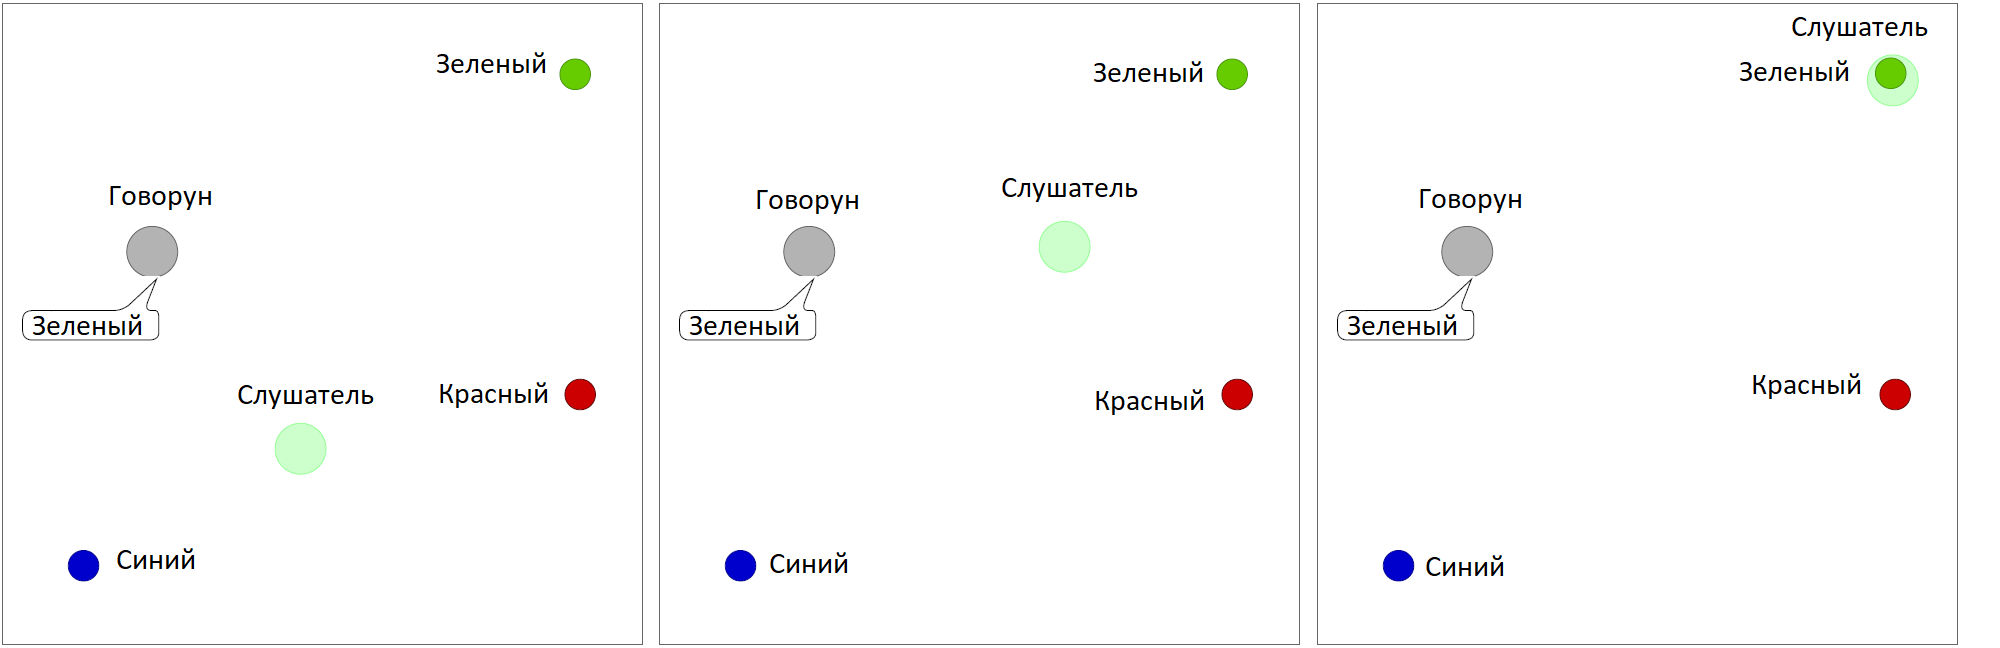
\includegraphics [scale=0.41] {my_folder/images/intro/ssl.png}
	\caption{Сценарий 1. \textit{Simple Speaker Listener}. Скриншоты слева направо показывают этапы игрового эпизода. \textit{Говорун} (серый) выдаёт коммуникационное действие, представляющее «зелёный», а \textit{слушатель} слушает сообщение \textit{говоруна} и направляется к цели}
	\label{fig-intro-ssl}
\end{figure}

\begin{figure}[ht!] 
	\center
	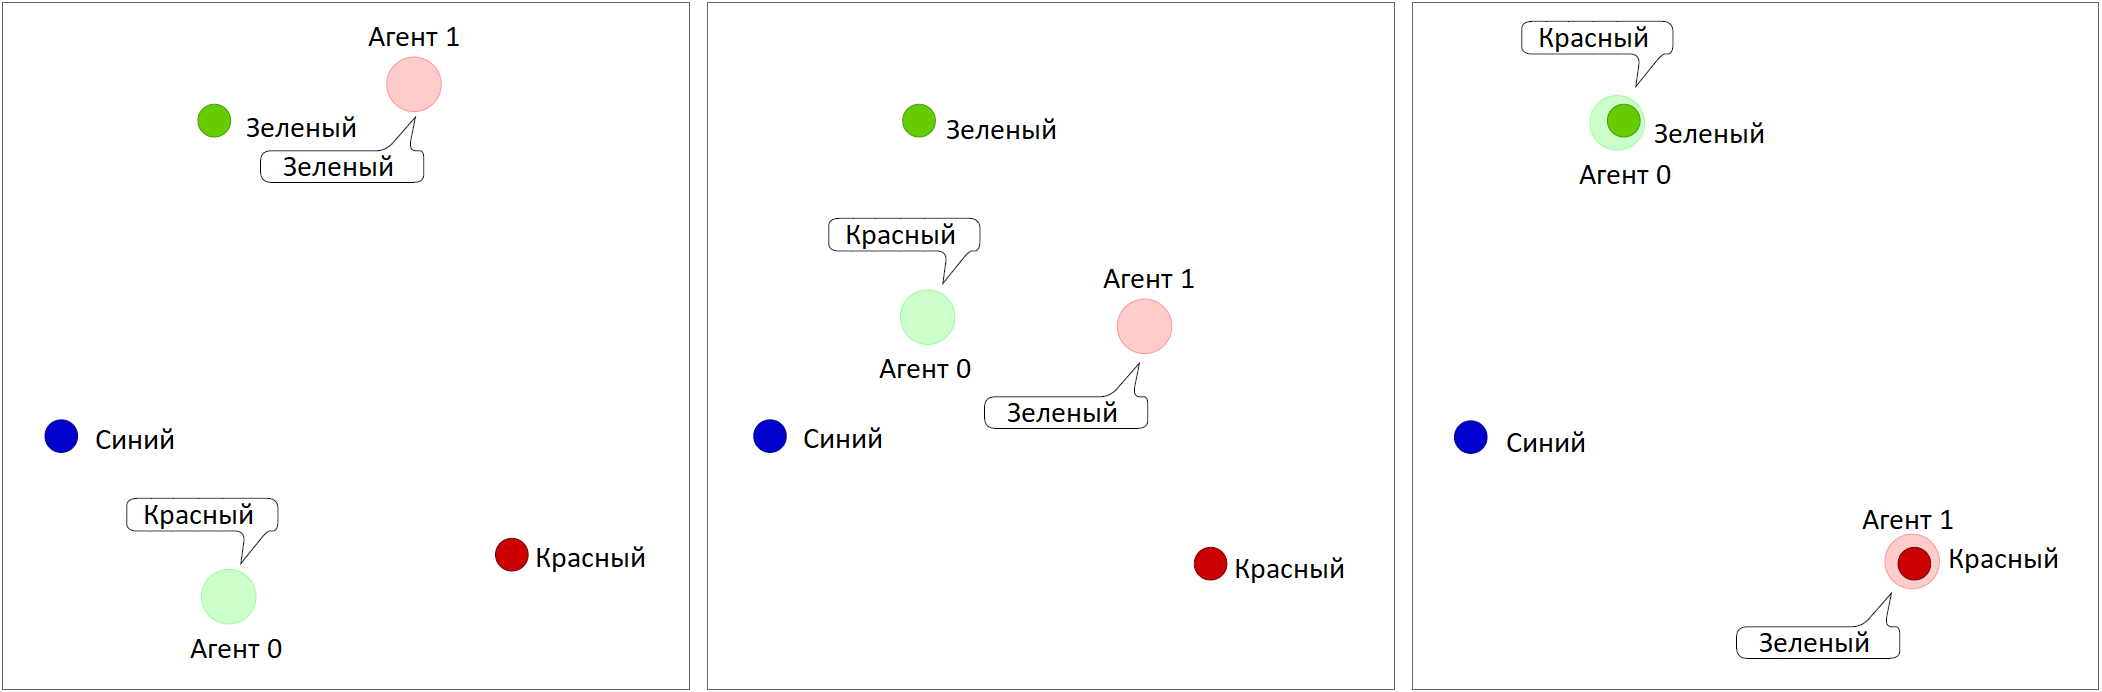
\includegraphics [scale=0.38] {my_folder/images/intro/sr.png}
	\caption{Сценарий 2: \textit{Simple Reference}. В этом эпизоде агент 0 (отображаемый в том же цвете, что и его целевой ориентир) выдаёт коммуникационное действие, представляющее «красный», и слушает агента 1. А агент 1 (отображается в том же цвете, что и его целевой ориентир) слушает и издаёт «зелёный» для Агента 0. Скриншоты слева направо показывают, как ведут себя два агента в соответствии с оптимальными политиками, слушая друг друга и перемещаясь к целям}
	\label{fig-intro-sr}
\end{figure}

\subsection{Сценарий 2. Simple Reference} \label{intro-sr}

Этот сценарий расширяет предыдущий, поскольку оба агента являются одновременно и \textit{говорунами} и \textit{слушателями}. Ориентиры остаются прежними, отображаются как три разноцветных объекта, (как изображено на \firef{fig-intro-sr}). Каждый из двух агентов пытается достичь своего целевого ориентира, который известен только другому агенту. Таким образом, он должен научиться сообщать другому агенту его цель и перемещаться к своей собственной. Что отличает сценарий от двух копий сценария \textit{Simple Speaker Listener}, так это то, что единое общее вознаграждение, присуждаемое агентам, основано на общей производительности. Таким образом, агенты должны выяснить, что идёт хорошо, а что нет. Настройка среды подробно описана в разделе \hyperref[exp-sr]{Эксперименты: Сценарий 2. Simple Reference}.
 % TODO: сверить имя главы

\subsection{Сценарий 3. Simple World Communication} \label{intro-swc}

В этом сценарии есть \textit{хорошие агенты} (зелёные) и их противники – \textit{преследователи} (красные). Также есть \textit{препятствия} (чёрные), \textit{леса} (зелёные) и \textit{еда} (зелёные). Один из преследователей – \textit{лидер} (тёмно-красный).

\textit{Хорошие агенты} награждаются за то, что приближаются к \textit{еде} и наказываются, когда касаются преследователей.

\textit{Преследователи} награждаются за касание хороших агентов.

\textit{Лес} скрывает агентов от преследователей. \textit{Лидер} видит агентов даже в лесу (cм. \firef{fig:swc}).

\begin{figure}[ht!] 
	\center
	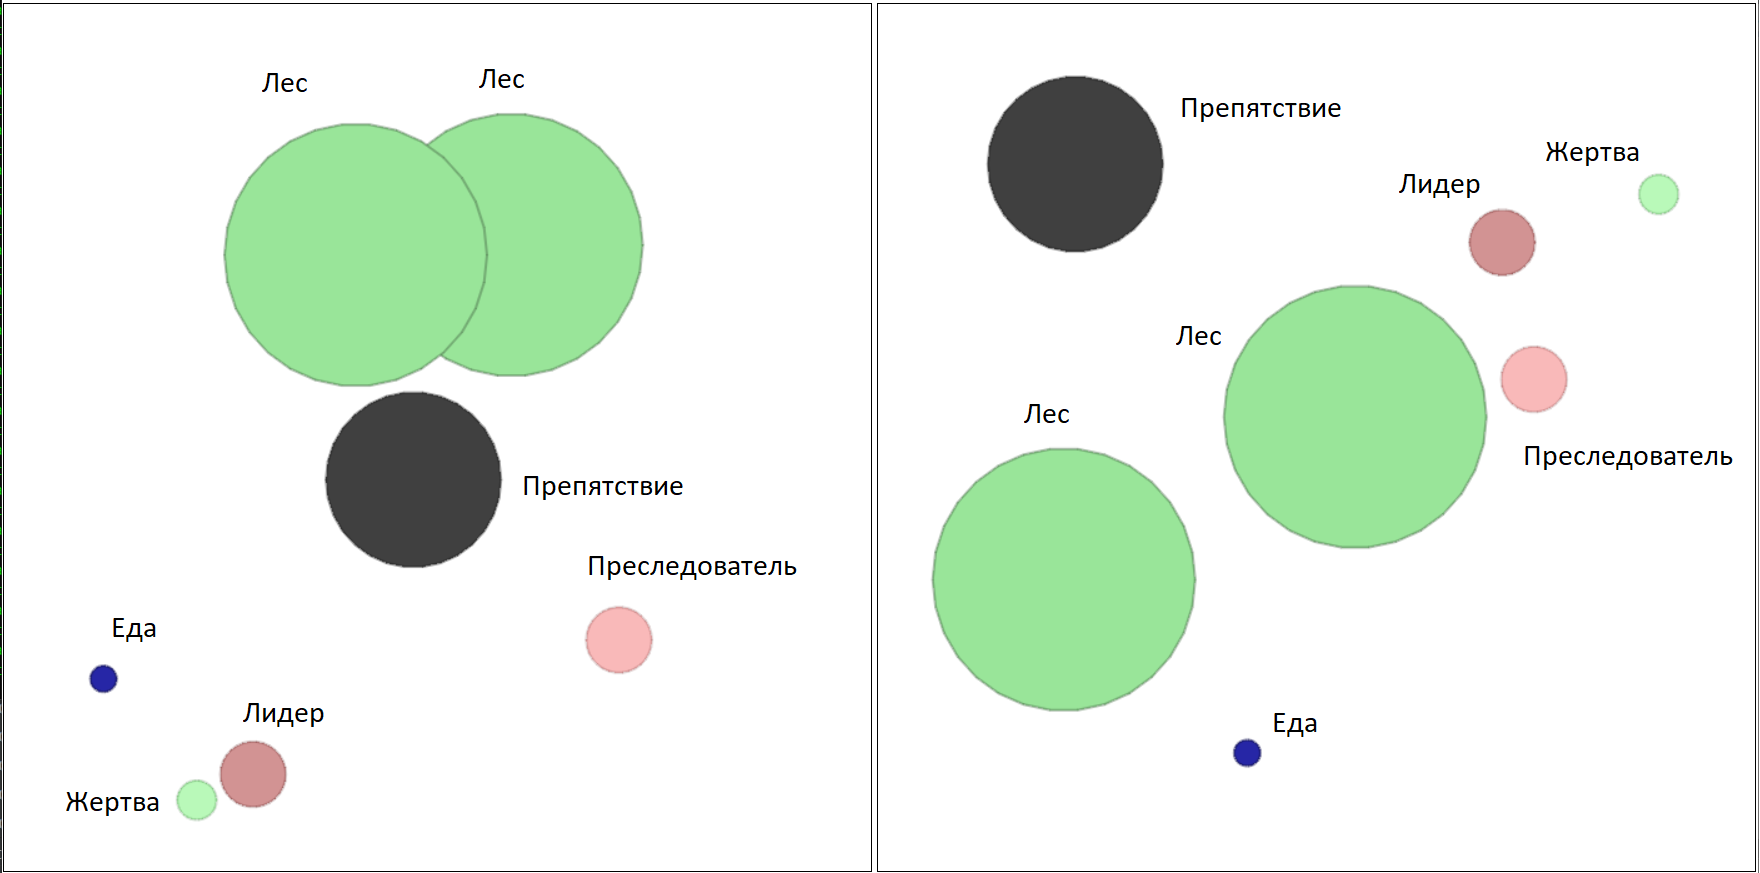
\includegraphics [scale=0.41] {my_folder/images/intro/swc.png}
	\caption{Сценарий Simple World Communication, жертва избегает преследователей, и, по возможности, приближается к еде, преследователи догоняют жертву}
	\label{fig:swc}  
\end{figure}

Более подробное описание и настройки можно найти в разделе \hyperref[exp-swc]{Эксперименты: Сценарий 3. Simple World Communication}.

\subsection{Сценарий 4: Simple Tag} \label{intro-st}

В этом сценарии есть \textit{хорошие агенты} (зелёные) и их противники – \textit{преследователи} (красные). Так же есть \textit{препятствие} (чёрное).

\textit{Хорошие агенты} наказываются, когда касаются \textit{преследователей}.

\textit{Преследователи} награждаются за касание \textit{хороших агентов}.

\textit{Преследователей} больше, но у \textit{жертвы} больше скорость. Теоретически, \textit{преследователи} должны выработать политику, при которой они окружают жертву или другие подобные приёмы. \textit{Жертва} должна не позволять загнать себя в угол.

Также мы немного модифицировали данный сценарий и добавили границу по периметру поля, которая не даёт агентам покинуть видимую часть.

\begin{figure}[ht!] 
	\center
	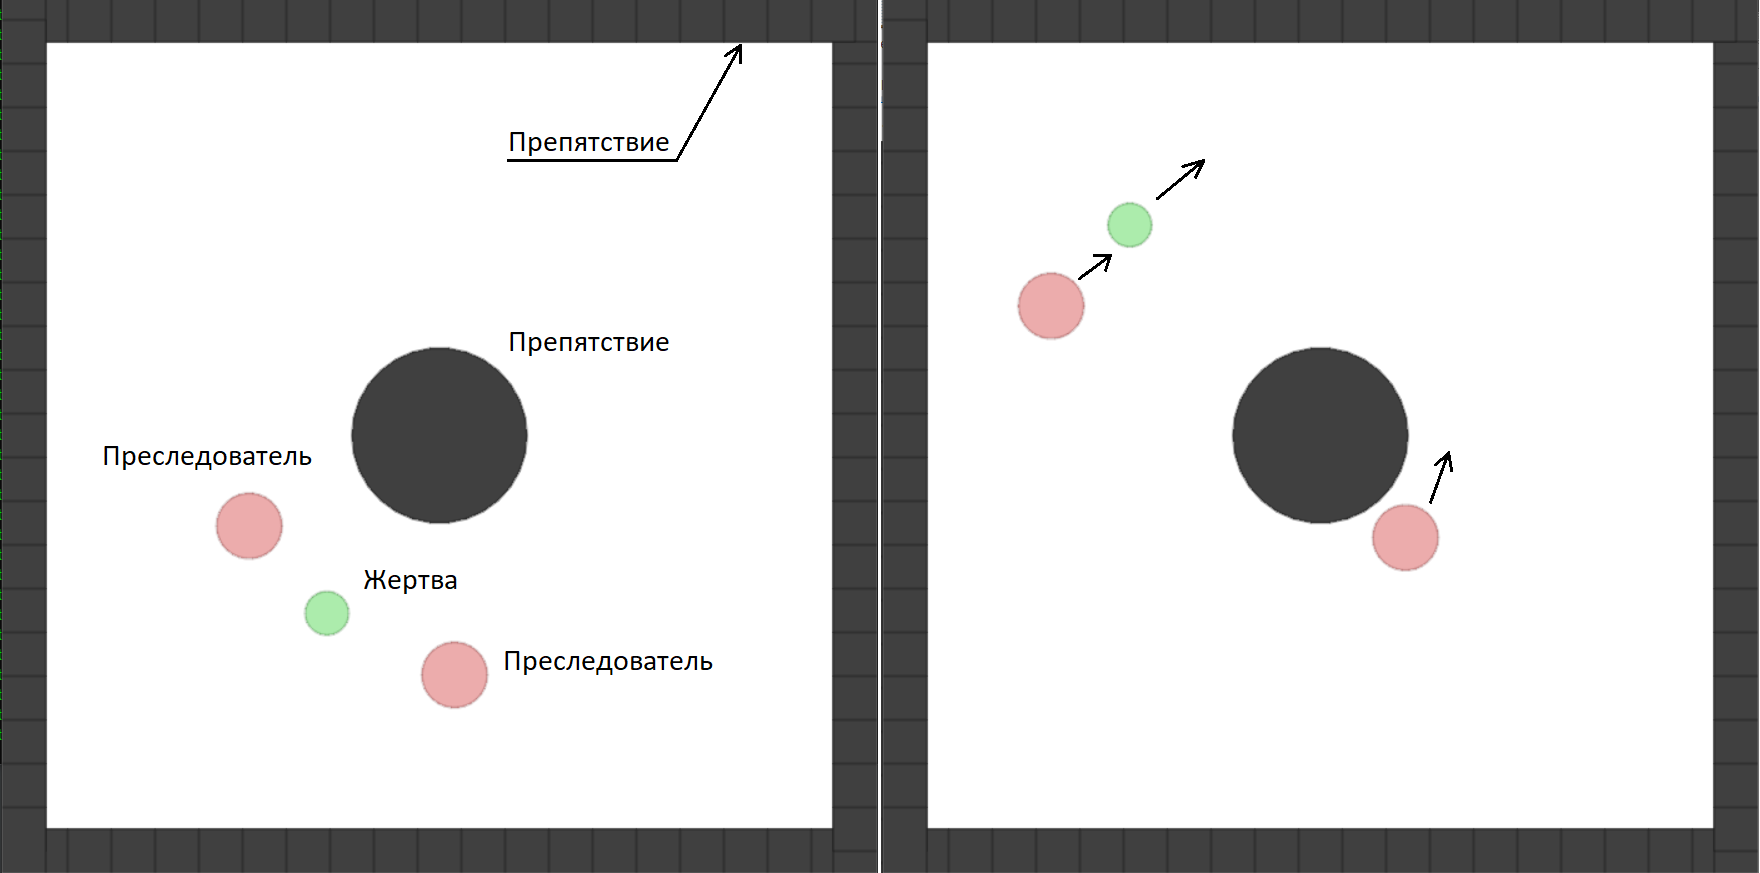
\includegraphics [scale=0.41] {my_folder/images/intro/st.png}
	\caption{Сценарий Simple Tag. \textit{Жертва} избегает \textit{преследователей}. На правом скриншоте правый преследователь превентивно обходит \textit{препятствие} справа и движется в ту же область, что и \textit{жертва}}
	\label{fig:st}  
\end{figure}

Более подробное описание и настройки можно найти в разделе \hyperref[exp-st]{Эксперименты: Сценарий 4. Simple Tag}.

\section{Практическая значимость} \label{intro:sec3}

Проект сосредоточен на обучении нескольких агентов совместной работе с использованием глубокого обучения в игровой среде. Результаты исследования могут быть дополнительно разработаны и широко использованы во многих практических реальных приложениях в области экономики, управления, техники и т.д. Например, он может применяться в робототехнике, к автономным транспортным средствам, производственным линиям, фондовым рынкам и т.д.

Перед применением в этих областях алгоритмы и методы, которые исследуются и разрабатываются в этой работе, должны быть хорошо протестированы и проверены, поскольку эти приложения непосредственно влияют на безопасность человека, социальную и финансовую безопасность. В долгосрочной перспективе применение мультиагентных алгоритмов приведёт к появлению всё большего числа автономных систем во многих областях.


%% Вспомогательные команды - Additional commands
%\newpage % принудительное начало с новой страницы, использовать только в конце раздела
%\clearpage % осуществляется пакетом <<placeins>> в пределах секций
%\newpage\leavevmode\thispagestyle{empty}\newpage % 100 % начало новой строки
	    	 % Введение

%% Начало основной части
\chapter{Обзор технологии обучения с подкреплением.} \label{ch1}

\section{Введение.} \label{ch1:intro}

Алгоритмы и методы глубокого обучения с подкреплением (Deep Reinforcement Learning, DRL) – это методы, которые мы используем для исследования вопросов дипломной работы. DRL – это подраздел машинного обучения, который лежит на пересечении Обучения с подкреплением (Reinforcement Learning) и глубокого обучения (Deep Learning). 

Прежде чем говорить о DRL, нужно кратко рассмотреть понятия, связанные с искусственным интеллектом и машинным обучением.

На \firef{fig:ch1-ML-and-AI-concepts} представлен обзор концепций, которые мы вводим в этой главе. 

Сначала мы рассмотрим искусственный интеллект, машинное обучение и его три категории. Затем мы углубимся в глубокое обучение. Наконец, мы рассмотрим основные алгоритмы DRL.
Таким образом, мы можем понять, почему и как DL и RL объединяются в DRL, который позволяет агентам взаимодействовать с более сложной средой и вести себя более разумно.

\begin{figure}[ht!] 
	\center
	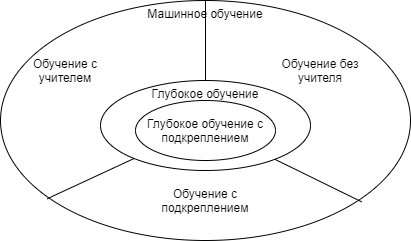
\includegraphics [scale=0.80] {my_folder/images/ch1/ML-and-AI-concepts.png}
	\caption{Граф, показывающий концепты МО и ИИ и их отношения.} 
	\label{fig:ch1-ML-and-AI-concepts}  
\end{figure}

\section{Искусственный Интеллект} \label{ch1:ai}

Искусственный интеллект \cite{Crevier93} (ИИ), как следует из названия, в отличие от естественного интеллекта человека и других животных, является искусственным. Именно такой тип интеллекта люди реализуют в машинах.
Конечной целью ИИ является создание таких автономных систем, которые способны учиться методом многочисленных проб и ошибок, чтобы найти оптимальное поведение для достижения максимально возможных целей в сложившемся окружении. \cite{RussellAndNorvig-AI-modern-approach}

С 21 века, благодаря нескольким прорывам, ИИ процветает в викторинах и настольных играх, превосходя уровень игры людей \cite{Watson} \cite{AlphaGo}. Наряду с увеличением вычислительной мощности, улучшения алгоритмов и доступности больших наборов данных, ИИ развивался революционными темпами. В ближайшем будущем, ИИ ещё сильнее повлияет на работу и повседневную жизнь человека.

\section{Машинное Обучение} \label{ch1:ml}

\subsection{Название первого подпараграфа первого параграфа первой главы для~демонстрации переноса слов в содержании} % ~ нужен, чтобы избавиться от висячего предлога (союза) в конце строки
\section{Глубокое обучение} \label{ch1:dl}

Глубокое обучение (Deep Learning, \hyperref[acr:dl]{DL})~--- подраздел машинного обучения, с применением которого в настоящее время достигаются выдающиеся результаты во многих областях, в том числе в распознавании изображений, компьютерном зрении, распознавании речи и обработке естесственных языков. Глубокое обучение как бы имитирует биологический мозг, обрабатывает информацию с помощью искусственных нейронных сетей.

Идея симуляции работы нейронов мозга человека зародилась десятилетия назад. Тем не менее, прорыв произошёл в последние годы, когда стали доступны большие наборы данных и вычислительные мощности \cite{10.1145/2771283}. Теперь можно строить модели с большим количеством слоёв искусственных нейронов, чем когда-либо прежде. Сети достигают исключительной производительности в области распознавания изображений и речи при значительном увеличении глубины. Считается, что глубокое обучение является одним из наиболее перспективных подходов для решения текущих задач ИИ.

\subsection{Искусственная нейронная сеть}

Мозг человека и животных~--- чрезвычайно сложный орган, который до сих пор до конца не изучен. Тем не менее, некоторые аспекты его структуры и функции были расшифрованы. Фундаментальным рабочим элементом в мозге является нейрон. Многочисленные нейроны связаны между собой сложным образом, что даёт возможность запоминания, мышления и принятия решений.

Хотя нейроны сложны и функционируют разными способами, все они имеют некоторые базовые компоненты такие как: ядро, дендриты, аксон и синапсы. Дендриты действуют как входные каналы, через которые нейроны получают информацию от синапсов других нейронов. Затем ядро обрабатывает эти сигналы и превращает в вывод, который затем отправляется в другие нейроны. Связь этих компонентов играет роль линии передачи в нейронных сетях.

Хоть \hyperref[acr:ann]{ИНС} и не так сложны, как человеческий мозг, они имитируют базовую структуру, которая включает входные, выходные слои, а также, обычно, скрытые слои. В каждом слое есть искусственные нейроны. Нейроны в одном слое обычно связаны с каждым нейроном в следующем слое. Они передают числовые сигналы через соединения с другими нейронами, примерно, как это происходит в биологической нейронной сети \cite{296402}.

Поскольку выходные сигналы нейронов ИНС представляются в виде вещественных чисел, выход обычно сравнивается с порогом. Только в том случае, если порог превышен, нейрон передаёт сигнал следующим подключённым нейронам.

\begin{figure}[ht!]
    \center
    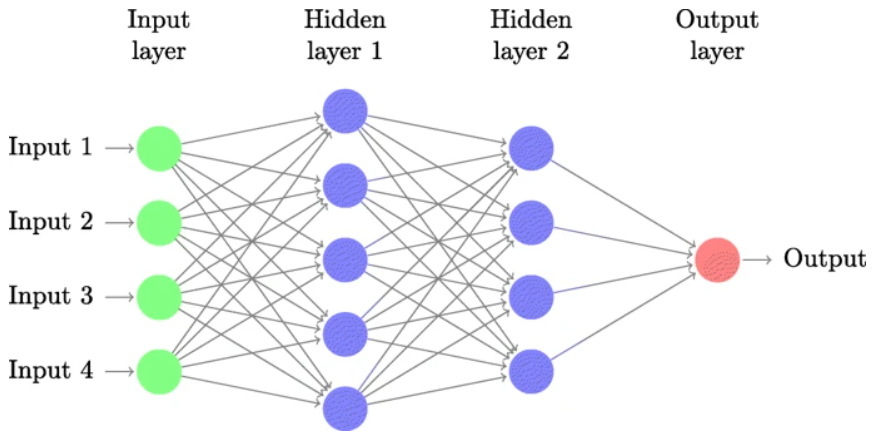
\includegraphics [scale=0.60] {my_folder/images/ch1/ANN.png}
    \caption{Базовая структура ИНС. ИНС обычно состоит из входного и выходного слоёв, а также пары скрытых слоёв. Основано на \cite{Khajanchi2003ArtificialNN} \cite{mitchell1997machine}}
    \label{fig:ch1-ANN}
\end{figure}

Связи между нейронами параметризованы весами, которые обновляются во время обучения, чтобы отрегулировать мощность сигналов, проходящих через сеть [24]; \firef{fig:ch1-ANN} показывает базовую структуру ИНС.

\subsection{Глубокая нейронная сеть}

Как уже упоминалось выше, концепция нейронной сети не нова.

На ранних этапах из-за ограничений вычислительной мощности, нейронные сети имели очень малую глубину. Обычно они содержали только входной, выходной слои и пару скрытых слоёв. Кроме того, количество нейронов в каждом слое также было ограничено. Глубокие нейронные сети не находили практического применения до последних лет, когда стали доступны огромные вычислительные мощности и большие объёмы данных.

Глубокие нейронные сети с несколькими слоями хороши для извлечения скрытых свойств \cite{7344858}. Каждый слой решает свою собственную задачу. Узлы в каждом слое учатся на конкретных наборах свойств, которые приходят из предыдущего слоя. Теоретически, чем глубже нейронная сеть, тем более сложны и абстрактны особенности, которые она может распознать, поскольку каждый нейрон агрегирует выводы из нейронов предыдущего слоя \cite{bengio2012representation}. Например, в задаче распознавания изображений вход представляет собой матрицу пикселей. Первый слой извлекает начальные объекты, такие как рёбра из пикселей, затем следующий слой кодирует расположение краёв и следующий слой распознаёт глаза, рот, уши, ноги, крылья, хвост и т.д. Наконец, последний слой распознаёт на изображении кошку, собаку или птицу. Таким образом, глубокие нейронные сети не нуждаются во вмешательстве людей, а сами изучают иерархию объектов.

С математической точки зрения нейронная сеть определяет функцию ${y = f(x; \theta)}$. Она описывает соответствие входных данных ${x}$ выходным ${y}$, где ${y}$ --- это категория в задаче классификации или выходное значение в задачах регрессии. Тренировка модели с использованием набора данных ведёт к вычислению параметра {$\theta$}.

После завершения обучения предполагается, что нейронная сеть аппроксимирует целевую функцию ${f^*}$ \cite{Goodfellow-et-al-2016}. Правильно обученная ИНС может лучше соответствовать набору данных, а также делает прогноз, учитывая неочевидные зависимости от данных.

Глубокие нейронные сети могут быть реализованы по-разному в зависимости от конкретных практических задач. Например, свёрточные нейронные сети специализируются на компьютерном зрении, а рекуррентные нейронных сети лучше подходят для обработки естественного языка.

Функцию отображения ${f(x)}$ можно рассматривать как цепочку из многих связанных функций в виде  ${f(x) = f^{(n)}(f^{(n-1)}(...f^{(2)}(f^{(1)}(x))))}$; ${n}$ связанных функций соответствуют глубине ИНС. Функция стоимости определяется на основе сравнения вывода ${y}$ из ${f(x)}$ с целевым значением ${t}$ из тренировочного набора данных. Цель обучения нейронной сети состоит в том, чтобы приблизить ${f(x)}$ функцей, минимизирующей функцию стоимости. Минимизация функции стоимости является задачей оптимизации, и для этого часто используют алгоритм {\itshape градиентного спуска}. В {\itshape обратном распространении} (backpropagation) градиент используется для итеративного обновления нейронной сети во время обучения. Оптимизатор решает, какие параметры и как должны быть обновлены, а {\itshape скорость обучения} (learning rate) задаёт размер шага, на который параметр обновляется на каждой итерации.

\section{Обучение с подкреплением} \label{ch1:rl}

Хотя алгоритмы \hyperref[acr:rl]{RL} эффективно решают различные задачи, им не хватает масштабируемости и размерности.

С ростом глубоких нейронных сетей в последние годы обучение с подкреплением начинает использовать их функции приближения и представления свойств \cite{HORNIK1991251}. Это помогает преодолеть недостатки алгоритмов обучения с подкреплением.

Это устраняет необходимость описывать свойства вручную, позволяя обучать модели, способные непосредственно выводить оптимальные действия, на основе необработанного и высокоразмерного ввода с сенсоров. Это проиллюстрировано на \firef{fig:DRL-flow}.

\begin{figure}[ht!]
    \center
    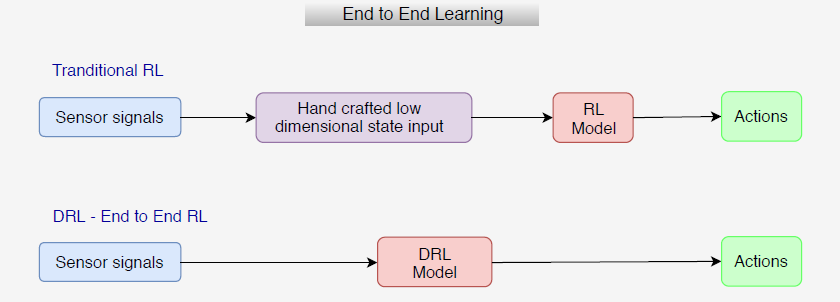
\includegraphics [scale=0.65] {my_folder/images/ch1/DRL-flow.png}
    \caption{Cравнение DRL и традиционной RL, где необходимо явно указать, какие действия производить в каких состояниях. Использование глубокой нейронной сети в DRL позволяет обучаться и принимать решения на основе необработанного сенсорного ввода}
    \label{fig:DRL-flow}
\end{figure}

Таким образом, использование ИНС в обучении с подкреплением создаёт новую область – глубокое обучение с подкреплением (Deep Reinforcement Learning, DRL).

\subsection{Алгоритмы глубокого обучения с подкреплением}

Два основных подхода к обучению с подкреплением: основанные на value-функции и на градиенте политики. Q-обучение~--- вероятностный value итерационный метод, цель которого~--- оценка Q-функции. Методы градиента политики же стараются оптимизировать политику напрямую.

Здесь нужно рассказать о \hyperref[acr:mdp]{марковском процессе принятия решений} (Markov Decision Process, MDP).

\subsubsection{Марковский процесс принятия решений}

Свойство Маркова означает, что следующее состояние зависит только от текущего состояния, тем самым, при принятии решения, можно игнорировать все прошлые состояния и учитывать только текущее.

Процесс {\itshape обучения с подкреплением} является формой \hyperref[acr:mdp]{МППР}. Он состоит из нескольких элементов:

\begin{itemize}
    \item набор состояний окружающей среды $S$;
    \item набор действий $A$;
    \item динамика перехода $T(s_{(t+1)}|s_t, a_t)$, которая описывает распределение новых состояний $s_{t+1}$, в которые может попасть агент, совершив действие $a_t$ в состоянии $s_t$;
    \item функция награды $R(s_t; a_t; s_{t+1})$;
    \item дискаунт фактор $\gamma \in [0, 1]$ для экспоненциального снижения будущих наград.
\end{itemize}

Политика $\pi$ сопоставляет состояниям распределение вероятностей принятия действий: ${\pi : S \to p(A = a|S)}$.

Эпизод~--- это предопределённый период времени, когда среда, начиная со случайного состояния, порождает серию переходов. Переходы в эпизоде можно рассматривать как траекторию политики.

Сумма наград, собранных в траектории политики: ${R = \sum_{t=0}^{T-1} \gamma^t r_{t+1}}$.

Цель обучения с подкреплением состоит в том, чтобы получить оптимальную политику ${\pi^*}$, которая максимизирует ожидаемую награду из всех состояний: ${\pi^* = argmax_x \mathbb{E} [R|\pi]}$ \cite{Otterlo2012ReinforcementLA}.

\subsection{Подход, основанный на функции состояния (Value Based подход)}

Этот подход состоит в том, чтобы оптимизировать значение функции $V(s)$.

Value-функция~--— это функция, которая сообщает нам максимальное ожидаемое будущее вознаграждение, которое агент получит в каждом состоянии. Значение каждого состояния — это общая сумма вознаграждений, на которую агент может рассчитывать в будущем, начиная с этого состояния.

\subsubsection{Q-обучение}

Функция состояния-значения (state-value function) $V^\pi (s) = \mathbb{E}[R|s, \pi]$~--- ожидаемая награда с данными состоянием $s$ и политикой $\pi$. В то же время в RL такой переход $T$ не всегда возможен, поэтому обычно используется другая функция состояния-значения или функция качества ${Q^\pi(s,a) = \mathbb{E}[R|s, a, \pi]}$. Оптимальная политика получается через выбор на каждом шаге действия, которое максимизирует Q-функцию \cite{SuttonAndBarto-RL-Introduction-p107}. Q-обучение~--- это алгоритм без политики (off-policy), так как он жадно выбирает действие исходя из текущего состояния, вместо того, чтобы следовать политике.

Для рекурсивного вычисления $Q^\pi$ применяется {\itshape уравнение Беллмана}:

\begin{equation}
    \label{eq:q-learning-bellmanEq}
    Q^\pi(s_t, a_t) = \mathbb{E}_{s_{t+1}}[r_{t+1} + \gamma Q^\pi (s_{t+1}, \pi(s_{t+1}))].
\end{equation}

Традиционное Q-обучение способно сформулировать оптимальную политику обучением состояние-действие-значение функции. Однако, оно предназначено для дискретных пространств действий с малым количеством измерений и не способно решать более-менее сложные задачи.

\subsubsection{Глубокая Q-сеть (DQN)}

Глубокая Q-сеть (DQN)~--- вариант Q-обучения, который использует глубокую сверточную нейронную сеть для вычисления Q-функции. Является прорывом в обучении с подкреплением. \cite{bertsekas1996neuro}

DQN была применена в игре Atari и достигла производительности, сопоставимой с человеческим уровнем. \cite{Mnih2015}

Для решения проблемы нестабильности и расхождения нелинейных функций аппроксиматоров, таких как нейронные сети, был применён метод {\itshape Experience Replay} [17]. Идея Experience Replay состоит в том, чтобы равномерно рандомизировать предыдущие переходы при обучении модели, что нарушает корреляцию последовательности наблюдений. Опыт агента ${e_t = (s_t, a_t, r_t, s_{t+1)}}$ на каждом шаге $t$ сохраняется в буфер ${D_t = ({e_1, ..., e_t})}$. Во время тренировки модели случайным образом извлекается небольшая часть опыта ${(s; a; r; s') \sim U(D)}$.

Еще одно новое приложение в DQN заключается в том, что создаются две Q-сети.
Текущая Q-сеть $Q(s, a; \theta_i)$ обновляется итеративно во время обучения, а целевая Q-сеть $Q(s', a'; \theta_i)$ используется для получения целевого Q-значения и обновляется только периодически. Целевая Q-сеть уменьшает смещение, вызванное неточностями Q-сети в начале обучения.

На каждой итерации $i$ Q-сеть обновляется на ошибку темпоральной разницы (temporal difference, TD):
\begin{equation}
    \label{eq:someEq}
    L_i(\theta_i) = \mathbb{E}_{(s, a, r, s') \sim U(D)} [(r + \gamma \max_{a'} Q(s', a'; \theta_i^-) - Q(s, a; \theta _i))].
\end{equation}

Где $\gamma$~--— это скорость затухания для будущих наград. $\theta _i^-$ параметры целевой Q-сети, и $\theta_i$~---текущей Q-сети на итерации. $[(r + \gamma \max_{a'} Q(s', a'; \theta_i^-)]$~--- это цель Беллмана при данной оценке $\theta_i^-$.

DQN для решения проблемы извлечения низкоразмерных свойства из высокомерного необработанного сенсорного сигнала, такого как пиксели изображения в играх, были применены глубокие нейронные сетеи. Тем не менее, он всё ещё ограничен его дискретным и низкоразмерным пространством действий.

\subsection{Линия поведения (Policy Based)}

Вместо получения оптимальной политики путём поддержания Q-функции, алгоритм напрямую ищет оптимальную политику путём максимизации ожидаемого значения $\mathbb{E}[R|\pi_\theta]$. Необходимо итеративно подгонять параметр $\theta$ сети так, чтобы максимизировать $\mathbb{E}[R|\pi_\theta]$.

В основном используется оптимизация, основанная на градиенте, так как это более эффективно при работе с большими сетями со множеством параметров. \cite{Arulkumaran_2017}

\subsubsection{Градиент политики (Policy Gradients)}

В методах, основанных на градиенте политики, параметризованную политику представляет нейронная сеть, которая обновляется при изучении сигналов. В обучении с подкреплением без модели для оценки градиента на примерах, сгенерированных в траектории политикой, используется правило {\itshape REINFORCE} или функция оценки. Предположим, что $f(х)$ – это функция оценки, где $x$~--- случайная величина для одного перехода. Градиент политики может быть рассчитан с использованием отношения правдоподобия:

\begin{equation}
    \label{eq:ch1-likelihood-ratios}
    \begin{multlined}
        \nabla_\theta \mathbb{E}_x[f(x)] = \mathbb{E}_x[f(x) \nabla_\theta \log p x|\theta].
    \end{multlined}
\end{equation}

Теперь рассмотрим траекторию $\tau$ с переходами $(a_t, s_t, r_t, s_{t+1})$ в соответствии с политикой, тогда градиент политики~--- это:

\begin{equation}
    \label{eq:ch1-likelihood-ratios}
    \begin{multlined}
        \nabla_\theta \mathbb{E}[R_\tau] = \mathbb{E}[\sum_\tau R_\tau \nabla_\theta \log \pi {a_\tau|s_\tau;\theta}].
    \end{multlined}
\end{equation}

Недостатком policy gradient является низкая скорость работы~—-- требуется большое количество вычислений для подсчёта награды. Также policy gradient может <<застрять>> в локальном оптимуме, не найдя глобального.

\subsubsection{Актор-критик}

Так как value-функция может предоставить обучающие сигналы для прямого поиска оптимальной политики, естественным было объединить два подхода.

В DRL две нейронные сети, представляющие актора и критика соответственно, используются для приближения функции, где актор (политика) учится по Q-значениям, оценённым критиком (value-функция) \cite{Arulkumaran_2017}. На \firef{fig:ch1-RL-actor-critic} показано, как актор и критик сети взаимодействуют с окружающей средой.

\begin{figure}[ht!]
    \center
    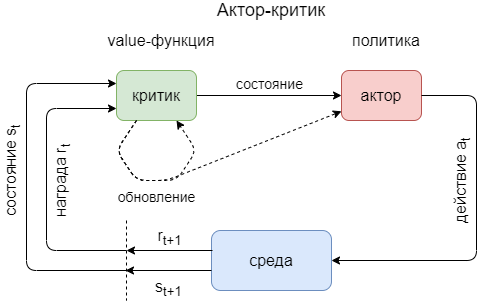
\includegraphics [scale=0.60] {my_folder/images/ch1/RL-actor-critic.png}
    \caption{{\itshape Актор} получает состояние из окружающей среды и реагирует на действие, {\itshape критик} получает состояние и награду и рассчитывает TD ошибку для обновления себя и {\itshape актора}. Основано на \cite{Arulkumaran_2017}}
    \label{fig:ch1-RL-actor-critic}
\end{figure}

\subsubsection{Глубокий детерминированный градиент политики (DDPG)}

\hyperref[acr:ddpg]{DDPG}~--- это актор-критик алгоритм, в котором нет модели и нет политики \cite{lillicrap2015continuous}. Он расширяет \hyperref[acr:dpg]{DPG} использованием глубоких нейронных сетей. Также, он использует хорошо зарекомендовавший себя приём DQN с текущей и целевой Q-сетями (сети критиков) и experience replay, чтобы стабилизировать обучение. И, наконец, он использует детерминированную политику (сеть акторов) вместо политики стохастического поведения.

В отличие от стохастической политики, которая определяет вероятность распределения через действия в данном состоянии, детерминированность в DDPG подразумевает, что конкретное действие аппроксимируется в данном состоянии. Соответственно конкретное состояние для следующего шага, также детерминировано.

Следовательно, вместо использования рекурсивного программирования, как в уравнении {\itshape Беллмана}, используется детерминированная политика ${\mu : S \leftarrow A}$ \cite{lillicrap2015continuous}

\begin{equation}
    \label{eq:ch1-ddpg-1}
    \begin{multlined}
        Q^\mu (s_t, a_t) = \mathbb{E}_{r_t, s_{t+1}~E}[r(s_t, a_t) + \gamma Q^\mu(s_{t+1}, \mu(s_{t+1})],
    \end{multlined}
\end{equation}
что очень похоже на Q-обучение – алгоритм с жадной политикой. Сеть критика обновляется по функции потерь

\begin{equation}
    \label{eq:ch1-ddpg-1}
    \begin{multlined}
        L(\theta^Q) = \mathbb{E}[(Q(s_t, a_t|\theta^Q) - y_t)^2],
    \end{multlined}
\end{equation}
где

\begin{equation}
    \label{eq:ch1-ddpg-3}
    \begin{multlined}
        y_t = r(s_t, a_t) + \gamma Q(s_{t+1}, \mu(s_{t+1})j\theta^Q).
    \end{multlined}
\end{equation}

Сеть актора обновляется функцией потерь

\begin{equation}
    \label{eq:ch1-ddpg-4}
    \begin{multlined}
        \nabla_{\theta \mu} J \approx \mathbb{E}[\nabla_{\theta \mu} Q(s, a \theta^Q)|_{s=s_t,a=\mu(s_t|\theta^\mu)}] = \\
        = \mathbb{E}[\nabla_a Q(s, a \theta^Q)|_{s=s_t,a=\mu(s_t) \nabla_{\theta \mu} \mu (s|\theta^\mu)|s=s_t}].
    \end{multlined}
\end{equation}

Как и в DQN, чтобы избежать расхождения, в DDPG применяется мягкое обновление (soft update) для целевых сетей критика и актора. Они обновляются только раз в указанное количество шагов.

	         	 % Глава 1
\ContinueChapterBegin % размещать главы <<подряд>>
\chapter{Обучение мультиагентных систем} \label{ch2}

\section{Введение} \label{ch2:intro}

В этой главе мы хотели бы представить соответствующую работу по теме «Мультиагентное глубокое обучение с подкреплением». Прежде всего, мы ссылаемся на современные алгоритмы, которые соответствуют нашим мультиагентным сценариям.

\section{Мультиагентные алгоритмы} \label{ch2:ma-algs} %название по-русски

Методы обучения с подкреплением, которые специализируются на решении задач с одним агентом, плохо адаптированы для многих реальных задач, таких как автономные транспортные средства, управление водоразделом, согласованный поиск объектов, управление городским траффиком, тороговля на фондовом рынке. Поэтому необходимо расширить эти алгоритмы или даже создать новые для более сложных сценариев с настройками для нескольких агентов.

Некоторые алгоритмы, которые вдохновили эту работу, иллюстрируются в следующих разделах. Этими алгоритмами являются Multi Agent Deep Deterministic Policy Gradient \cite{lowe2017multiagent}, Counterfactual baseline for multi-agent policy gradient \cite{foerster2017counterfactual} и emergent grounded compositional language \cite{mordatch2017emergence}.

\subsection{Детерминированная политика для нескольких агентов}

Multi Agent Deep Deterministic Policy Gradient (\hyperref[acr:maddpg]{MADDPG}) --- это расширение \hyperref[acr:ddpg]{DDPG}, применяемое к настройкам нескольких агентов. Чтобы учесть все состояния среды и политики всех агентов RL в игровом сценарии, алгоритм учитывает совместные наблюдения и действия всех агентов при обучении сетей акторов и критиков. Когда дело доходит до принятия решения, сеть актора каждого агента учитывает только локальные наблюдения. Эта структура централизованного обучения и децентрализованного исполнения позволяет каждому агенту вычислять оптимальную политику по консистентному градиентному сигналу. \cite{lowe2017multiagent}

\begin{figure}[ht!]
    \center
    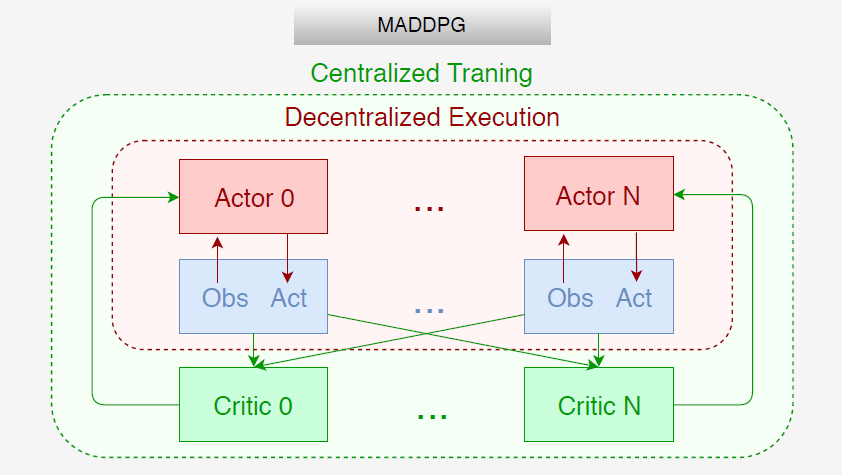
\includegraphics [scale=0.80] {my_folder/images/ch2/maddpg.png}
    \caption{У каждого агента есть децентрализованная сеть акторов, которая получает доступ только к своим локальным наблюдениям. Между тем, каждый агент имеет централизованную сеть критиков, которые имеют доступ к наблюдениям и действиям всех агентов. Критик сети обучен обновлять себя и актора. Основано на \cite{lowe2017multiagent}}
    \label{fig:ch2-maddpg}
\end{figure}

Совместные наблюдения всех агентов обозначаются через $\mathbf{x} = (o_1, ..., o_N)$, совместные действия --- через $a = (a_1, ..., a_N)$. Они вместе с наградами $r$ хранятся в буфере $D$ в виде $(\mathbf{x}, a, r, \mathbf{x}')$. Случайная выборка из $S$ выборок $(\mathbf{x}^j, a^j, r^j, \mathbf{x}'^j)$ извлекается из $D$, а \textit{критик} каждого агента обновляется путём минимизации потерь:

\begin{equation}
    \begin{multlined}
        L(\theta_i) = \dfrac{1}{S} \sum_j (y^j - Q_{i}^\mu (\mathbf x^j, a_{1}^j, ...,a_{N}^j))^2
    \end{multlined}
\end{equation}.

И \textit{актор} обновляется семплированым градиентом политики:

\begin{equation}
    \begin{multlined}
        \nabla_{\theta_i} J \approx \dfrac{1}{S} \sum_j \nabla_{\theta_i} \mu_i (o^j_i) \nabla_{a_i} Q^\mu_i (x^j, a^j_1, ..., a_i, ..., a^j_N)|_{a_i=\mu_i(o^j_i)}
    \end{multlined}
\end{equation}.

Подобно DDPG, целевые сети обновляются «мягко» на каждом шаге на $\theta' \leftarrow \tau \theta + (1 - \tau) \theta'$ с $\tau \ll 1$.

Алгоритм MADDPG хорошо подходит для сценариев с физической навигацией. Было решено продолжить изучение этого алгоритма с помощью многомерного пространства действий, Он хорошо подходит для сценариев, в которых агенты могут взаимодействовать при выполнении физических действий.

\subsection{Контрафактный мультиагентный градиент политики (Counterfactual Multi-Agent Policy Gradient, COMA)}

Контрфактический мультиагентный градиент политики (\hyperref[acr:coma]{COMA}) - это мультиагентный вариант метода \textit{актор-критик}, который использует единого централизованного \textit{критика} для приближения к Q-функции и отдельных децентрализованных \textit{акторов} для оптимизации политики каждого агента $\pi (h)$. \cite{foerster2017counterfactual}

В кооперативных задачах с несколькими агентами сложность сотрудничества возрастает с увеличением количества агентов. Таким образом, было бы нецелесообразно и неэффективно иметь одну единственную оптимальную политику для всех агентов. Вместо этого децентрализованные политики для каждого агента формулируются в виде проблем с несколькими агентами. В COMA один централизованный критик и отдельные акторы тренируются на совместных действиях и совместных наблюдениях. Когда дело доходит до исполнения, каждый актор генерирует действия на основе собственной истории наблюдения $h$, см. \firef{fig:ch2-coma}.

\begin{figure}[ht!]
    \center
    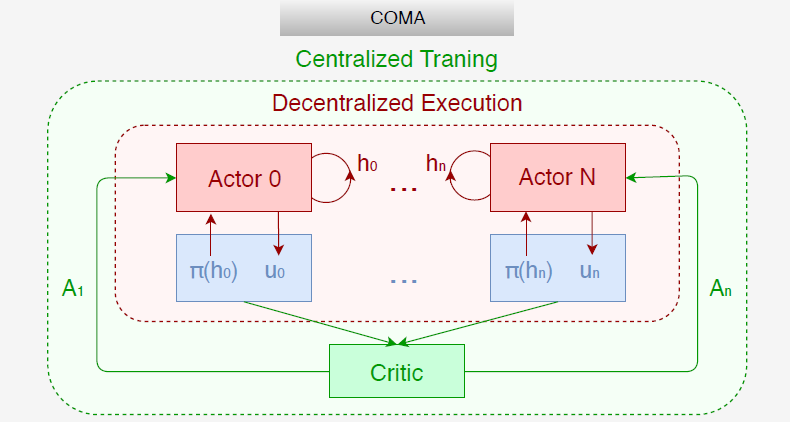
\includegraphics [scale=0.80] {my_folder/images/ch2/coma.png}
    \caption{Структура сетей алгоритма COMA и информационный поток между централизованным критиком и децентрализованными акторами. В COMA отдельно происходит обучение одного централизованного критика и каждого из акторов. Каждый актор децентрализован, при принятии решений использует локальную историю наблюдения $h$ \cite{foerster2017counterfactual}}
    \label{fig:ch2-coma}
\end{figure}

COMA предназначен для мультиагентных совместных сценариев с глобальной функцией награды для всех агентов. Однако агенты, обученные COMA, изучают отдельные политики без явного общения. \cite{foerster2017counterfactual}

\subsection{Возникающий язык (Emergent Language)}

Grounded compositional language обозначает простой язык, где агенты связывают конкретные символы с конкретными объектами, а затем объединяют эти символы в значимые понятия \cite{Szabo2008-SZAC}. Язык представлен в виде абстрактных дискретных символов, произнесённых агентами, которые не имеют заранее определённого значения, но возникли и сформировались в процессе обучения в соответствии со средой и целями \cite{mordatch2017emergence}. В отличие от естественного языка, для работы с которым извлекаются языковые шаблоны из большого набора текстовых данных, этот язык, возникший во время обучения с подкреплением, понятен только агентам и используется ими для сотрудничества друг с другом в достижении общих целей.

\section{Действия и награды} \label{ch2:act-rew} %название по-русски

\subsection{Архитектура ветвления действий (Action Branching)}

Обычно довольно трудно исследовать проблемы с многомерными пространствами действий. Архитектура \textit{ветвления действий} предназначена для решения таких проблем. Например, в среде с \textit{N}-мерным пространством действий и $d_n$ дискретных последующих действий для каждого измерения \textit{n} необходимо рассмотреть в общей сложности $\Pi^N_{n=1} d_n$ возможных действий \cite{tavakoli2017action}. Правильно спроектированные разветвленные архитектуры действий могут эффективно и результативно исследовать такое большое многомерное пространство действий \cite{tavakoli2017action}.

\begin{figure}[ht!]
    \center
    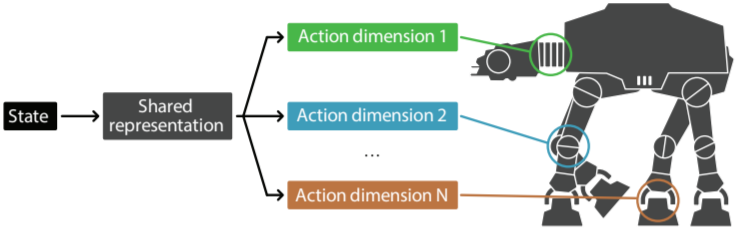
\includegraphics [scale=0.80] {my_folder/images/ch2/action-branching.png}
    \caption{Архитектура сети для ветвления действий, например, для робота, где сеть принимает состояние в качестве входных данных и разделяет нижние уровни для извлечения представлений признаков, а затем расходится по ветвям для относительно независимых под-действий, включая, например, высказывание, действие рукой, действие ногой и т. д. Основано на \cite{tavakoli2017action}.}
    \label{fig:ch2-action-branching}
\end{figure} % TODO: перевести

Основной идеей архитектуры является модуль совместного принятия решений, который извлекает скрытое представление из входного наблюдения и создает отдельные выходные ветви для каждого измерения действия. На рисунке \firef{fig:ch2-action-branching} представлена архитектура \textit{ветвления действий}. \textit{n} измерений действий представляют собой \textit{n} относительно независимых под-действий.
В архитектурах \textit{ветвления действий} значения \textit{Q} рассчитываются для каждого измерения действия. Тем не менее, мы бы хотели, чтобы многомерное действие оценивало одно единственное \textit{Q}-значение, выводимое сетью критика.

\subsection{Архитектура гибридного вознаграждения} % TODO: "Декомпозированная награда"?

Как показано в \cite{seijen2017hybrid}, жизненно важно иметь точную оптимальную value-функцию в обучении с подкреплением, поскольку она оценивает ожидаемый return как сигнал для оптимизации политики. Как только оптимальная value-функция изучена, из неё можно получить оптимальную политику.

\begin{figure}[ht!]
    \center
    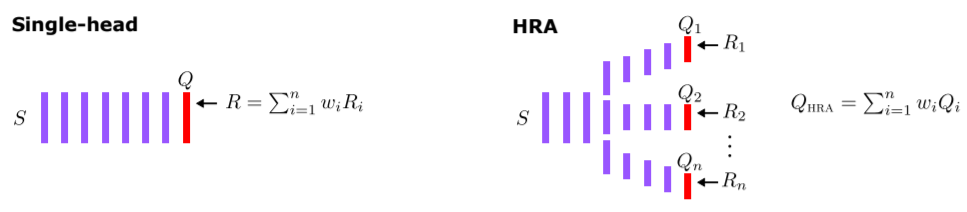
\includegraphics [scale=0.80] {my_folder/images/ch2/hybrid-reward.png}
    \caption{Глубокая нейронная сеть с одной головой, аппроксимирует одну единственную Q-функцию с глобальной функцией награды (слева), и Q-сеть с гибридной архитектурой вознаграждения (справа). Сеть имеет n голов, аппроксимирующих n Q-функций. Каждая Q-функция оценивает Q-значение с помощью соответствующей разложенной функции награды. Основано на \cite{seijen2017hybrid}.}
    \label{fig:ch2-hybrid-reward}
\end{figure} % TODO: перевести

Более того, две разные value-функции могут привести к одной и той же политике, когда агент действует жадно в соответствии с ними \cite{seijen2017hybrid}. Следовательно, можно было бы изучить несколько более простых value-функций, если изучить сложную value-функцию сложно или даже невозможно. В таком случае глобальная функция награды может быть соответственно разложена на несколько различных функций награды:

\begin{equation}
    \begin{multlined}
        R_{rev}(s, a, s') = \sum^n_{k=1} R_k (s, a, s')
    \end{multlined}
\end{equation}

где $R_{rev}$ - глобальная функция награды, которая разбита на \textit{n} функций награды. Каждая разложенная функция награды зависит от подмножества состояний и имеет свою собственную функцию \textit{Q}-значения. Глубокая \textit{Q}-сеть с общими нижними слоями и \textit{n} головами используется для аппроксимации \textit{n} \textit{Q}-значений, обусловливающих текущее состояние и действие с различными функциями разложения награды \firef{fig:ch2-hybrid-reward}.

\begin{equation}
    \begin{multlined}
        Q_{H R A}(s, a; \theta) := \sum^n_{k=1} Q_k(s, a;\theta)
    \end{multlined}
\end{equation}

Q-сеть затем итеративно улучшается за счет оптимизации функции потерь

\begin{equation}
    \begin{multlined}
        L_i(\theta_i) = \mathbb{E}_{s, a, r, s'}[\sum^n_{k=1}(y_{k, i}-Q_k(s, a;\theta_i))^2]
    \end{multlined}
\end{equation}

где

\begin{equation}
    \begin{multlined}
        y_{k, i} = R_k(s, a, s') + \gamma \max_{a'} Q_k(s', a';\theta_{i-1})
    \end{multlined}
\end{equation}

$\theta_i$ — это веса Q-сети в текущей итерации \textit{i}, а $\theta_{i-1}$ - веса отдельной целевой сети в предыдущей итерации.
В гибридной архитектуре вознаграждений \textit{n} \textit{Q}-значений выводятся \textit{n} головами из одной единственной \textit{Q}-сети. Однако для того, чтобы иметь консистентный градиент для улучшения политики для каждого измерения действий, следует создавать отдельные \textit{Q}-сети для оценки \textit{Q}-значений для каждого измерения действий.


\section{Учебная программа}

Обучение по \textit{учебной программе} — это стратегия обучения, основанная на процессе обучения человека. В системе образования люди обучаются путём ознакомления с концепциями, которые строятся от простых до сложных уровней, от конкретных до более абстрактных уровней, от простых структур до сложных модулей.

Машинное обучение заимствует такой подход. \textit{Учебная программа} усложняет обучение программы от небольших подзадач или простых аспектов к более тяжёлым и сложным задачам. Ожидается, что обученная модель достигнет высокой эффективности и результатов обучения \cite{10.5555/3171837.3172051}.

В методе \textit{учебная программа} простой аспект проблемы проливает свет на общую картину, а сложные факторы постепенно добавляются и раскрывают больше деталей целой картины. Поиск решения для сглаженной версии проблемы и затем переход к более детализированной может помочь обучению решить проблему постепенно \cite{graves2017automated}.

Математически $C_\gamma (\theta)$ определяется как функции стоимости задачи, в которой $\gamma$ - уровень сложности, а $\theta$ - параметры. Начальную сглаженную версию $C_0$ обычно легко оптимизировать, доведя $\theta$ до локального минимума. Локальный минимум затем используется в качестве основы для следующего уровня сложности. С увеличением $\gamma$, $C_\gamma$ становится менее сглаженной при дальнейшем поиске следующего локального минимума на основе предыдущего локального минимума. \cite{10.1145/1553374.1553380}

Учебный план также можно рассматривать как последовательное пере-взвешивание, в начале на наборах данных из простых примеров, а затем на полном наборе данных. С увеличением уровня сложности в набор обучающих данных добавляются немного более сложные примеры, которые используются для повторного взвешивания распределения. В конце используется полный набор обучающих данных. \cite{10.1145/1553374.1553380}

\newpage % принудительное начало с новой страницы, использовать только в конце раздела
	         	 % Глава 2
\chapter{Применяемые методы} \label{ch3}

Основным алгоритмом, применяемым в этой работе, является \hyperref[acr:ddpg]{\textit{градиент глубокой детерминированной политики}} (Deep Deterministic Policy Gradient, DDPG), который использует архитектуру актор-критик и может работать в пространстве непрерывных действий. Поскольку сценарий игры предполагает совместную работу нескольких агентов, используется мультиагентная модификация алгоритма DDPG - \hyperref[acr:maddpg]{\textit{мультиагентный градиент глубокой детерминированной политики}} (MADDPG). Основное его отличие, делающее его более подходящим для работы с несколькими агентами, состоит в том, что MADDPG имеет N наборов ИНС критиков-акторов, где N соответствует количеству агентов в сценарии, благодаря чему, каждый агент имеет свой собственный механизм оптимизации политики. В оригинальном дизайне \cite{lowe2017multiagent} это сделано для адаптации как к совместной работе, так и к конкуренции между агентами.
Поскольку эта ВКР фокусируется на совместной работе нескольких агентов, тестируются несколько вариантов MADDPG, подходящих для совместной работы. % TODO: в разработке

\section{Основные методы}

\subsection{Архитектура актор-критик}

Как уже упоминалось выше, алгоритм MADDPG имеет набор сетей актор-критиков для каждого агента в игровой среде. Для облегчения многоагентной совместной работы, во время тренировки, алгоритм учитывает наблюдения и действия всех агентов. Политики оптимизируются путём оценки качества, поведения всех агентов в разных состояниях среды. Таким образом, в условиях среды, требующей взаимодействия агентов, будет разработана политика, оптимальная для сотрудничества.

Глубокая нейронная сеть может рассматриваться как аппроксиматор нелинейных функций. В решении сложных задач глубокого обучения с подкреплением нейронная сеть нестабильна \cite{lillicrap2015continuous}. Эту проблему решает использование целевой (target) сети, поскольку мягкое и разрежённое обновление целевой сети замедляет её приближение к исходной сети и уменьшает влияние ошибок. Таким образом, это нарушает корреляцию между текущими и целевым Q-значениями. Хотя это снижает скорость обучения, но и улучшает стабильность обучения. В алгоритме MADDPG и у актора, и у критика есть свои целевые сети.

\subsection{Воспроизведение опыта (Experience Replay)}

Воспроизведение опыта — это механизм, когда во время тренировки в игровой среде буфер используется для сбора опыта, образцы которого из этого буфера затем случайным образом извлекаются для обучения модели.

Опыт генерируется последовательно, во время взаимодействия агентов со средой в хронологическом порядке. Неизбежно то, что собранные последовательности опыта коррелируют друг с другом. Из-за этого сеть легко переобучается на имеющиеся последовательности опыта. В итоге, переобученная сеть не может обеспечить разнообразный опыт для последующего обучения.

Опыт случайно отбирается в небольшие блоки. Это нужно не только для эффективного использования аппаратного обеспечения и увеличения скорости обучения, но также нарушает корреляцию последовательности в буфере. Таким образом, сети имеют возможность формулировать более обобщённые политики по независимым друг от друга данным.

Для применения воспроизведение опыта, в буфер, складывается опыт в виде кортежей переходов, включающих наблюдения, действия, награды и последующие наблюдения, то есть $e_t = (\mathbf{s, a, r, s'})$. Поскольку это многоагентная игровая среда, \textbf{s} - это совместные наблюдения, которые представляют собой совокупность наблюдений n агентов, $\mathbf{s} = [s_0, s_1, ..., s_n]$. То же самое относится к действиям, следующим наблюдениям и наградам. Буфер имеет ограниченную ёмкость, и при переполнении старый опыт вытесняется новым.

\subsection{Тренировка ИНС}

В то время, как агенты исследуют игровую среду, опыт перехода на каждом шаге собирается в буфер памяти. Обучение происходит только тогда, когда количество кортежей в буфере превышает определённую величину. Когда начинается обучение, \textit{актор} и \textit{критик} каждого из \textit{n} агентов обновляется на каждом шаге, в то время как \textit{целевой актор} и \textit{целевой критик} обновляются с задержкой (раз в определённое количество шагов).

На рисунке \firef{fig:ch3-network-training} показано, как обновляется набор сетей акторов-критиков. Текущее Q-значение $Q_i(\mathbf{s, a}|\theta ^Q_i)$ оценивается по сети \textit{критика}, при этом на вход подаются совместные текущие наблюдения \textbf{s} и совместные действия \textbf{a}. Целевое Q-значение $y_i$ рассчитывается из вознаграждения и дисконтированного следующего Q-значения $Q'_i(\mathbf{s', a'}|\theta ^{Q'_i})$ аппроксимированного по \textit{целевому критику}. Входные данные для сети \textit{целевого критика} – это совместные последующие наблюдения \textbf{s}' из буфера и совместные последующие действия \textbf{a}', оценённые \textit{целевыми} сетями \textit{акторов}:

\begin{equation}
    \begin{multlined}
        \mathbf{a'} = [a'_0, a'_1, ..., a'_n] \\
        = [\mu'_0(s'_0|\theta^{\mu'_0}), \mu'_1(s'_1|\theta^{\mu'_1}), ..., \mu'_n(s'_n|\theta^{\mu'_n})]
    \end{multlined}
\end{equation}

Целевое Q- значение:

\begin{equation}
    \begin{multlined}
        y_i = r_i + \gamma Q'_i(\mathbf{s', a'}|\theta^{Q'_i})
    \end{multlined}
\end{equation}

где $r_i$ это награда – \textit{i}-го агента, и $\gamma$ - это коэффициент дисконтирования или скорость затухания влияния будущих наград.

Наконец, сеть \textit{критика} обновляется путём минимизации функции потерь:

\begin{equation}
    \begin{multlined}
        L_i(\theta^{Q_i}) = \frac{1}{S} \sum (y_i - Q_i(\mathbf{s, a}|\theta^{Q_i}))^2
    \end{multlined}
\end{equation}

где \textit{S} -- это размер тренировочного набора.

\begin{figure}[ht!]
    \center
    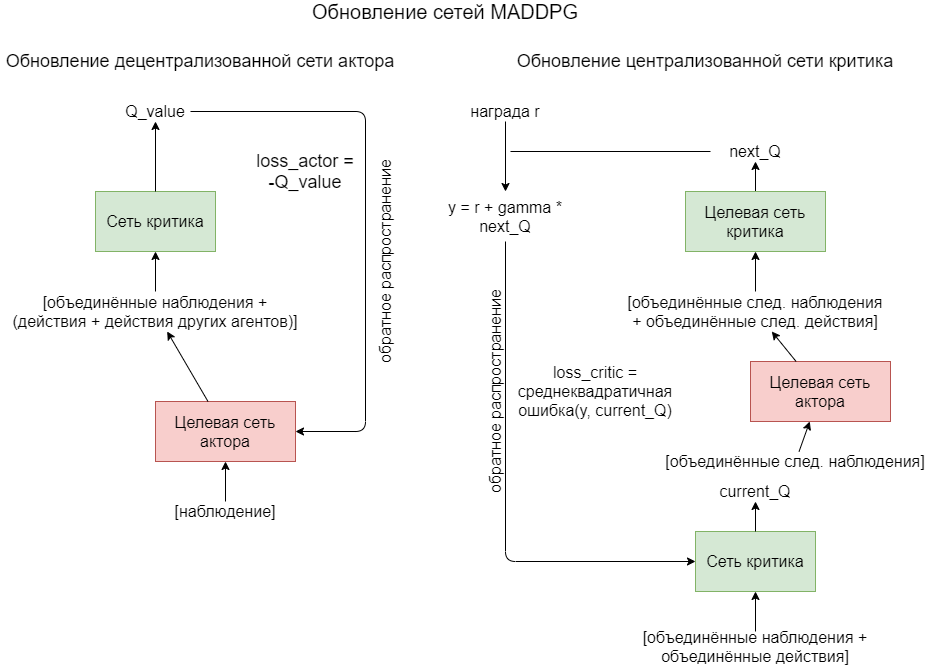
\includegraphics [scale=0.5] {my_folder/images/ch3/maddpg-updating-networks.png}
    \caption{Обновление сети \textit{актора} и \textit{критика} для каждого агента в MADDPG}
    \label{fig:ch3-network-training}
\end{figure}

Сеть \textit{актора} \textit{i}-го агента обновляется путём максимизации Q-значения сетью \textit{критика}. \textit{Критик} принимает совместные текущие наблюдения \textbf{s} из буфера и совместные текущие действия, в которых \textit{i}-е действие подменяется последним действием оценённым \textit{актором}. То есть:

\begin{equation}
    \begin{multlined}
    [a_0, a_1, a_i, ..., a_n]
        = [a_0, a_1, \mu_i(s_i|\theta^{\mu_i}), ..., a_n]
    \end{multlined}
\end{equation}

Для оптимизации уместно преобразовать задачу максимизации в задачу минимизации. Следовательно, функция потерь для обновления сети актора:

\begin{equation}
    \begin{multlined}
        L_i(\theta^{\mu_i}) = -Q_i(\mathbf{s}, [a_0, a_1, \mu_i(s_i|\theta^{\mu_i}), ..., a_n]|\theta^{Q_i})
    \end{multlined}
\end{equation}

Сети \textit{целевых актора} и \textit{критика} обновляются не полным копированием сетей \textit{актора} и \textit{критика}, а с использованием \textit{мягкого обновления} (soft update):

\begin{equation}
    \begin{multlined}
        \theta^{\mu'_i} = \tau \theta^{\mu_i} + (1 - \tau)\theta^{\mu'_i}\\
        \theta^{Q'_i} = \tau \theta^{Q_i} + (1 - \tau)\theta^{Q'_i}
    \end{multlined}
\end{equation}

где $\tau$ обычно очень мала, например 0.01 в этой работе.

\section{Прикладные методы}

\subsection{Архитектура ветвления действий (Action Branching)}

В сценариях, подразумевающих совместную работу нескольких агентов наряду с физическими действиями важно иметь и коммуникационные действия. В некоторых случаях количество действий может быть большим, как в \cite{tavakoli2017action}. В игровых сценариях этой работы агент имеет два вида действия, которые представляют физическое движение и действие, выбранное для общения.

Полное действие в таких сценариях включает в себя два относительно независимых действия. Сеть \textit{акторов} проектируется таким образом, что она выделяет скрытые представления из наблюдений и имеет две «головы» на выходе. Одна возвращает физическое действие, вторая – действие для общения.

В соответствии с теорией архитектуры ветвления действий \cite{tavakoli2017action}, можно оптимизировать каждое измерение действия относительно независимо. Полное действие в итоге представляет собой объединение двух действий.

\subsection{Исследовательский шум (Exploration Noise)}

\textit{Исследование} и \textit{эксплуатация} (Exploration and exploitation) — это дилемма в обучении с подкреплением. \textit{Эксплуатация} — это когда агент следует текущей политике, чтобы совершать жадные действия, которые приносят наибольшую награду. \textit{Исследование} берет на себя риски, чтобы попробовать другие действия, которые потенциально могут принести лучшую награду в долгосрочной перспективе. \textit{Исследование} необходимо агенту, ищущему оптимальную политику, хотя оно кажется неоптимальным в нынешней ситуации и дает меньшее вознаграждение. В обучении с подкреплением агент обычно больше \textit{исследует} окружающую среду в начале обучения. В ходе оптимизации политики с течением времени, агент постепенно уменьшает и стабилизирует \textit{исследование} до низкого уровня, и в итоге больше придерживается получившейся оптимальной политики.

Чтобы включить \textit{исследование}, на действия накладываются шумы. Какой шум применять, определяется настройкой среды. \textit{Процесс Орнштейна-Уленбека} используется в DDPG в [2] для получения коррелированных по времени \textit{исследований}. Он считаются, эффективным для проблем физического контроля с инерцией. Гауссовское распределение шума используется для физических движений в [4]. В этой работе для наложения шума на действия, генерируемые сетью \textit{акторов} выбирается стандартное \textit{Гауссовское распределение}.

\begin{equation}
    \begin{multlined}
        \mu'_i(s_i) = \mu_i(s_i|\theta^{\mu_i}) + \mathcal{N}
    \end{multlined}
\end{equation}

где $\mu'$ - политика исследования, а $\mathcal{N}$ - шум исследования, который можно выбрать в зависимости от настроек среды. $\mathcal{N}$ затухает на каждом шаге со скоростью $\epsilon$, то есть $\mathcal{N} \leftarrow \epsilon \mathcal{N}$.

\section{Варианты алгоритмов}

\subsection{MADDPG с декомпозированным вознаграждением (Decomposed Reward)}

Предполагается сценарий игры, в котором агенты выполняют относительно независимые под-действия, каждое под-действие может воздействовать на среду и приводить к вознаграждению, которое отделено от глобального вознаграждения. Идея декомпозирования награды MADDPG в том, что для каждого под-действия может быть сформулирована независимая политика. Каждый агент, имеет \textit{n} независимых наборов сетей \textit{актор-критиков}, каждый из которых соответствует одному виду действия. Ожидается, что политики для отдельных видов действий могут быть оптимизированы путем обучения соответствующих групп критиков.

В этой работе планируется использовать этот вариант в сценарии \textit{Simple Reference}.

\subsection{MADDPG с общим мозгом}

Другой вариант MADDPG вдохновлен \cite{mordatch2017emergence}. В этом варианте есть только один набор сетей \textit{акторов-критиков}, который используется всеми агентами. Это подразумевает, что все агенты имеют одинаковую оптимальную политику. Этот подход использует предположение о том, что все агенты имеют одно и то же пространство действий и пространство наблюдений, и они также имеют общую глобальную награду. Этот подход особенно эффективен для коммуникационных действий, поскольку композиционный язык постоянно появляется среди всех участников игрового сценария. В варианте с общим набором сетей все агенты говорят на одном языке, в отличие от стандартного MADDPG, где каждый агент может интерпретировать один и тот же ориентир по-разному. Это особенно важно, когда сотрудничают более двух агентов, поскольку им нужно общаться на одном языке.


\newpage
           	 % Глава 3
\chapter{Сценарии и эксперименты}

Эксперименты проводятся в мультиагентной среде multiagent-particle-envs \cite{multiagent-particle-envs} от компании OpenAI.


\section{Эксперименты}

\subsection{Эксперимент на одном мозге}

В алгоритме MADDPG каждый агент имеет набор сетей \textit{критиков}, чтобы иметь собственный механизм оптимизации политики. Тем не менее, два агента в \textit{Simple Reference} полностью симметричны в том смысле, что они оба имеют одинаковое пространство наблюдения, пространство действий и имеют общую глобальную награду. Тем самым агенты формулируют аналогичные оптимальные политики.

Таким образом, каждому агенту можно было бы не создавать свой собственный мозг из сетей критиков, а вместо этого тренировать один мозг для всех агентов. Кроме того, единый мозг MADDPG позволяет агентам общаться на одном «языке», что означает, что они произносят и понимают ориентиры в одних и тех же кодировках.

Так же мы разработали вариант этого алгоритма, можно сказать, что в том случае мы имеем два мозга: один для агентов из одной команды, второй – для агентов из другой команды. Этот вариант мы применили к сценарию \textit{Simple Tag}. Это возможно благодаря тому, что агенты из одной команды в этом сценарии имеют одинаковое пространство наблюдения, пространство действий и имеют общую глобальную награду, но это не так для агентов из разных команд. Поэтому и пришлось использовать отдельный набор сетей для каждой команды.

\subsection{Эксперимент с декомпозированным вознаграждением}

Чтобы обеспечить чёткие сигналы для двух независимых поддействий, мы попробовали реализовать отдельные наборы \textit{актор-критиков} для физического движения и общения.

\begin{figure}[ht!]
    \center
    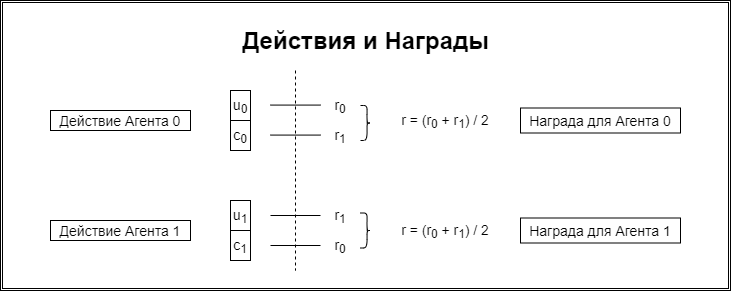
\includegraphics [scale=0.60] {my_folder/images/ch4/actions_and_rewards.png}
    \caption{С левой стороны от пунктирной линии - действие агента, которое представляет собой совокупность физического движения \textit{u} и коммуникационного действия \textit{c}. С правой стороны показано, как награда рассчитывается и назначается для оценки действий. Два агента имеют одинаковую глобальную награду - среднее значение между $r_0$ и $r_1$}
    \label{fig:action-reward}
\end{figure}

Из \firef{fig:action-reward} видно, что физическое перемещение $u_0$ агента 0 оценивается $r_0$, а высказывание $c_0$ - $r_1$. Окончательное вознаграждение затем раскладывается как кортеж из $r_0$ и $r_1$, т.е. $[r_0; r_1]$, причем каждый элемент соответствует сигналу оценки физического движения и связи соответственно. Точно так же последний набор вознаграждений для агента 1 равен $[r_1; r_0]$.

\begin{figure}[ht!]
    \center
    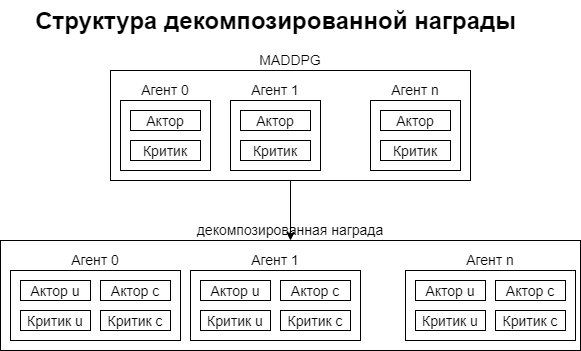
\includegraphics [scale=0.60] {my_folder/images/ch4/decomposed_reward_structure.png}
    \caption{Сетевая структура декомпозированного вознаграждения по сравнению со стандартным MADDPG}
    \label{fig:decomposed-reward-structure}
\end{figure}

Для физического движения и общения созданы два отдельных набора сетей \textit{актор-критик}, чтобы обеспечить согласованные и точные градиенты для оптимизации двух поддействий, см. \firef{fig:decomposed-reward-structure}. Разложения вознаграждения можно рассматривать как параллельное обучение двух слушателей из \textit{Simple Speaker Listener}. 1 - это агент 0 с коммуникацией $c_0$ в качестве говорящего и агент 1 с физическим движением $u_1$ в качестве слушателя, а 2 - агент 1 с c1 в качестве говорящего и агент 0 с $u_0$ в качестве слушателя, как показано на \firef{fig:action-reward}.

MADDPG с разложенным вознаграждением может быть хорошо приспособлен только к \textit{Simple Reference}, но не может быть обобщён для других игровых сценариев. Поскольку, пространства наблюдений и действий у агентов в этом сценарии симметричны, а главное, каждый агент производит оба вида действия. В большинстве других сценариев это не так. Следовательно, необходимо проводить больше экспериментов с общей глобальной наградой.

\subsection{Эксперимент с обучением по учебной программе}

Обучение по учебной программе применено с целью решения проблемы расходящихся сетей, возникшей в ходе обучения. Примеры обучения организованы в таком порядке, что постепенно вводятся все более сложные концепции.

Варианты учебной программы, на примере сценария Simple Reference:

\begin{itemize}
    \item увеличивать количество ориентиров постепенно. Первый уровень сложности в этой учебной программе с фиксированной целью для обоих агентов, скажем, красным ориентиром в качестве цели. На втором уровне добавляется ещё один ориентир, например зелёный, и цель выбирается случайным образом из двух ориентиров. Последний уровень - это исходная настройка сценария, т. е. рандомизация цели из трех ориентиров. Цель этой учебной программы состоит в том, чтобы агенты учились от простого сценария с меньшим количеством ориентиров к более сложному сценарию со всеми ориентирами;
    \item обучить агента 0 в качестве \textit{говоруна} и агента 1 в качестве \textit{слушателя} на первом этапе, а на следующем этапе обучить двух агентов в качестве \textit{говорунов} и \textit{слушателей} в исходном игровом сценарии;
    \item предоставить агентам заранее определенные коммуникационные действия для трёх цветов, скажем, [1; 0; 0] для красного, [0; 1; 0] для зелёного и [0; 0; 1] для синего. Таким образом, первая фаза состоит в том, чтобы изучить физическое движение, чтобы правильно двигаться. Затем, одному из агентов больше не предоставляются предопределённые коммуникационные действия, но взамен предоставляется связь с другим агентом (показываются его коммуникационные действия). Ожидается, что другому агенту будет легче научиться правильно общаться. Наконец, мы возвращаемся к исходным игровым настройкам для двух агентов, когда изучаются как физическое движение, так и общение.
\end{itemize}

TODO: каждый пункт - новое предложение?

\section{Метрики измерения консистентности коммуникационных действий}

Обучение модели можно ориентировочно оценивать на глаз при рендеринге физического движения, но можно и создать метрику и строить по ней графики. Выбранная метрика для коммуникационных действий заключается в том, что агент должен однозначно интерпретировать комунникационные действия и выбирать соответствующие им цвета цели.

Методика, используемая для измерения сходимости коммуникации, заключается в том, что мы создаем матрицу которая сопоставляет интерпретацию агента и текущий цвет цели. Допустим, строки – это цвета целей, а коммуникационные действия представлены в one hot encoded строках (строки, в которых максимальное значение в векторе действия представляется в виде 1, а остальные – 0). Тогда после нормализации матрицы, если обучение сходится, она должна выглядеть примерно так:

\begin{equation*}
    \begin{bmatrix}
        1 & 0 & 0 \\
        0 & 1 & 0 \\
        0 & 0 & 1
    \end{bmatrix}
\end{equation*}

или

\begin{equation*}
    \begin{bmatrix}
        1 & 0 & 0 \\
        0 & 0 & 1 \\
        0 & 1 & 0
    \end{bmatrix}
\end{equation*}

и т. д.

Не важно, как агенты интерпретируют цвета, \textit{детерминант} этой матрицы, в конце концов, стремиться к 1 или -1. Мы в своих экспериментах использовали этот способ.

Ещё один способ измерения заключается в том, чтобы смотреть, какое действие коммуникации выбрал говорун, при наблюдении определённого цвета и проверять, совпадает ли оно с тем, что было выбрано в прошлый раз с тем же наблюдением. График с результатом должен приблизиться к $100\%$ после схождения.

\section{Сценарии}

\subsection{Сценарий 1. Simple Speaker Listener}  \label{exp-ssl}

Сценарий Simple Speaker Listener воспроизводится и тестируется с использованием алгоритма MADDPG \cite{lowe2017multiagent}.

Сценарий упоминается в разделе \hyperref[intro:ssl]{Вводная глава: Сценарий 1. Simple Speaker Listener}. В этом сценарии два агента имеют разные пространства действий и наблюдений. Наблюдение говоруна $o_s$~--- это цвет цели, обозначенный 3- канальным вектором $d \in \mathbb{R}^3$. Наблюдение слушателя $o_l$ – это вектор конкатенации его собственной скорости $\upsilon \in \mathbb{R}^2$ его расстояния до трёх ориентиров $p = [p_1, p_2, p_3], p_i \in \mathbb{R}$ и сигнал, произнесённый говоруном на предыдущем временном шаге:

\begin{equation}
    \begin{multlined}
        o_s = [d], \\
        o_l = \begin{bmatrix}
                  \upsilon \\ p \\ c
        \end{bmatrix}.
    \end{multlined}
\end{equation}

Коммуникационное действие говоруна обозначается «one-hot encoding» вектором ${[1; 0; 0]}$, или ${[0; 1; 0]}$, или ${[0; 0; 1]}$ для обозначения трёх ориентиров соответственно.
Физическое действие u слушателя~--- это 5-канальный вектор, каждый из которых представляет одно направление движения (вверх, вниз, влево, вправо или без движения). Наблюдения и действия говоруна и слушателя и их взаимосвязь показаны на рисунке \firef{fig:ch4-ssl}.

\begin{figure}[ht!]
    \center
    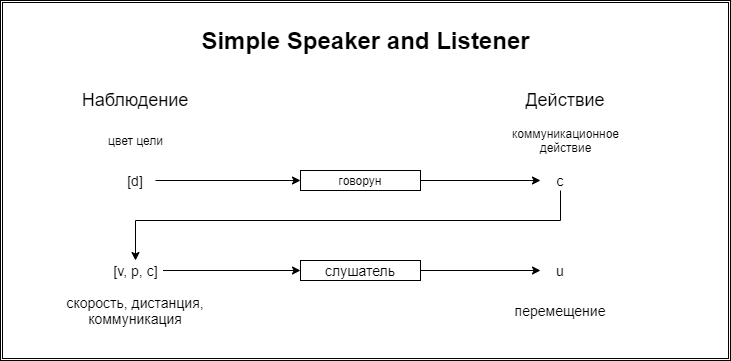
\includegraphics [scale=0.60] {my_folder/images/ch4/simple_speaker_listener.png}
    \caption{Говорун наблюдает цвет целевого ориентира d и издаёт коммуникационое действие, которое будет получено слушателем. Слушатель производит физическое движение}
    \label{fig:ch4-ssl}
\end{figure}

Два агента имеют общую награду r, которая является отрицательным евклидовым расстоянием между слушателем и его целью. Проблема, которую необходимо решить в этом сценарии, заключается в поиске оптимальных политик для говоруна и слушателя, чтобы максимизировать ожидаемую награду, то есть найти $\max_{\pi}R(\pi)$, где

\begin{equation}
    \begin{multlined}
        R(\pi) = \mathbb{E}[\sum_{t=0}^{T}r(s_t, a_t)].
    \end{multlined}
\end{equation}

Во время обучения говорун учится различать три ориентира и передавать целевой ориентир слушателю. И слушатель должен изучить закодированные высказывания говоруна и перейти к правильной цели.

Архитектура актор-сети говоруна аналогична архитектуре слушателя, каждый из которых содержит два полносвязанных слоя с 64 нейронами и использует функцию активации relu. Однако их выходные слои различаются с точки зрения количества единиц. Сети критиков имеют структуру, аналогичную сетям акторов, за исключением того, что они выдают скалярное Q-значение.

На этом сценарии было произведено измерение консистентности коммуникационных действий для алгоритмов DDPG и MADDPG.

\subsection{Сценарий 2. Simple Reference} \label{exp-sr}

Simple Reference~--- это более сложный сценарий, который расширяет Simple Speaker Listener.

Проблема, которую необходимо решить в этом сценарии, была изложена в разделе \hyperref[intro-sr]{Вводная глава: Сценарий 2. Simple Reference}. На \firef{fig-intro-sr} показан сценарий игры и поведение агентов при использовании оптимальных политик. В этом сценарии оба агента одновременно выступают и слушателями, и говорунами, что означает, что они оба выполняют как физические, так и коммуникационные действия. Высказывание каждого агента на одном шаге наблюдается другим агентом на следующем шаге, как показано на \firef{fig:exp-sr}.

Каждый агент наблюдает скорость, расстояние до ориентиров, цвет цели другого агента и высказывание другого агента. Действие каждого агента состоит из двух поддействий: физического движения $u$ и коммуникационного действия $c$.

Наблюдение и действие:

\begin{equation}
    \begin{multlined}
        o_i = \begin{bmatrix}
                  \upsilon \\ p \\ d \\ c
        \end{bmatrix}, \\
        a_i = \begin{bmatrix}
                  u \\ c
        \end{bmatrix}.
    \end{multlined}
\end{equation}


Это показано на \firef{fig:exp-sr}.

Наградой каждого агента является среднее значение отрицательных евклидовых расстояний от агентов до их целей. Таким образом, оцениваются как физические, так и коммуникационные действия агентов. Предположим, что $r_0$~--- это отрицательное евклидово расстояние от агента 0 до его цели, а $r_1$~--- это расстояние от агента 1 до его цели. Окончательная награда для каждого агента:

\begin{equation}
    \begin{multlined}
        r = \frac{r_0 + r_1}{2}.
    \end{multlined}
\end{equation}

Награда $r_0$ используется для оценки физического движения $u_0$ агента 0 и коммуникационного действия $c_1$ агента 1. То же относится и к $r_1$ - он используется для оценки физического движения $u_1$ агента 1 и высказывания $c_0$ агента 0. Это показано на \firef{fig:exp-sr}.

Архитектура нейронных сетей актора-критика двух агентов в этом сценарии аналогична архитектуре в предыдущем сценарии.

\begin{figure}[ht!]
    \center
    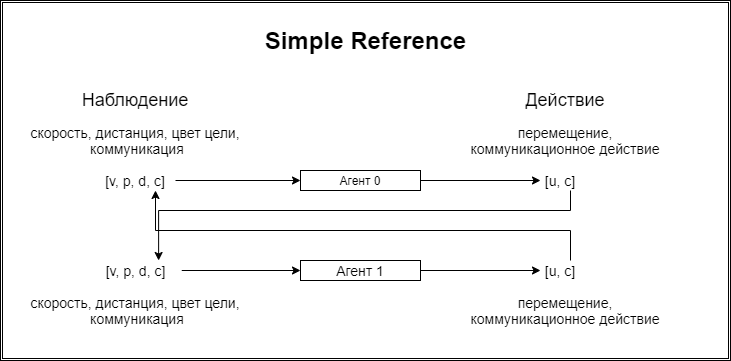
\includegraphics [scale=0.60] {my_folder/images/ch4/simple_reference.png}
    \caption{Каждый агент наблюдает целевой ориентир другого и производит коммуникационное действие, которое будет получено другим агентом на следующем шаге}
    \label{fig:exp-sr}
\end{figure}

В этом сценарии был поставлен эксперимент с декомпозированным вознаграждением, а также эксперимент с общим мозгом

Так же на этом сценарии производилось измерение консистентности коммуникационных действий.

\subsection{Сценарий 3. Simple World Communication} \label{exp-swc}

Кратко этот сценарий был описан в разделе \hyperref[intro-swc]{Вводная глава: Сценарий 3. Simple World Communication}. На \firef{fig:swc} показан сценарий игры и поведение агентов при использовании оптимальных политик. В этом сценарии лидер выступает говоруном, остальные преследователи – слушателями. И те, и другие перемещаются в погоне за хорошими агентами. Лидер выступает говоруном, а преследователи~--- слушателями. Высказывание лидера на одном шаге наблюдается другими преследователями на следующем шаге, как показано на \firef{fig:exp-swc}.

Хорошие агенты просто наблюдают еду и преследователей и перемещаются.

Под едой подразумевается объект, при приближении к которому, хорошие агенты получают награду

\begin{figure}[ht!]
    \center
    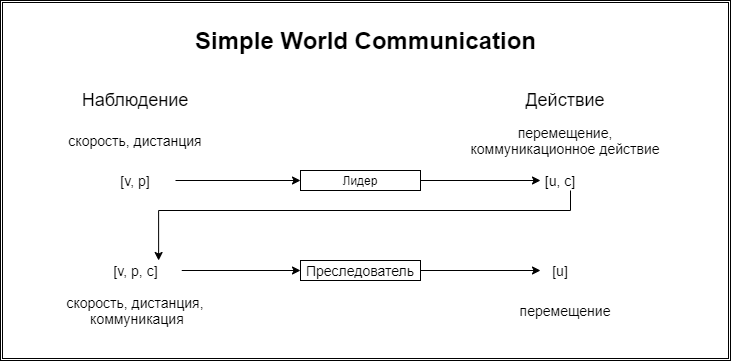
\includegraphics [scale=0.60] {my_folder/images/ch4/simple_world_communication.png}
    \caption{Лидер видит то, чего, возможно, не видят другие преследователи, и производит коммуникационное действие, которое будет получено преследователями на следующем шаге}
    \label{fig:exp-swc}
\end{figure}

Каждый преследователь наблюдает скорость $\upsilon \in \mathbb{R}^2$, расстояние до жертв $p = [p_1, p_2, p_3], p_i \in \mathbb{R}$, и высказывание лидера. Лидер наблюдает то же самое, кроме высказывания. Действие лидера состоит из двух поддействий: физического движения $u$ и коммуникационного действия $c$. Действие преследователя – только из физического движения $u$.
Наблюдение и действие лидера:

\begin{equation}
    \begin{multlined}
        o_i = \begin{bmatrix}
                  \upsilon \\ p
        \end{bmatrix}, \\
        a_i = \begin{bmatrix}
                  u \\ c
        \end{bmatrix}.
    \end{multlined}
\end{equation}

Наблюдение и действие преследователя:

\begin{equation}
    \begin{multlined}
        o_i = \begin{bmatrix}
                  \upsilon \\ p \\ c
        \end{bmatrix}, \\
        a_i = \begin{bmatrix}
                  u
        \end{bmatrix}.
    \end{multlined}
\end{equation}

Это показано на рисунке \firef{fig:exp-swc}.

Наградой каждого преследователя является отрицательное евклидово расстояние до ближайшего агента.

Во время обучения лидер учится, как закодировать положение жертвы, чтобы передать его преследователю. И преследователь должен изучить закодированные высказывания лидера и двигаться к жертве.

Архитектура нейронных сетей в этом сценарии аналогична архитектуре в предыдущем сценарии.

На этом сценарии производилось измерение консистентности коммуникационных действий.

\subsection{Сценарий 4: Simple Tag} \label{exp-st}

Кратко этот сценарий был описан в разделе \hyperref[intro-st]{Вводная глава: Сценарий 4. Simple Tag}. На \firef{fig:st} показан сценарий игры и поведение агентов при использовании оптимальных политик. В этом сценарии нет общения между агентами, но пространства наблюдения и действий всех преследователей совпадают, это позволяет применить к нему метод обучения с одним мозгом. В этом сценарии все агенты наблюдают друг друга и перемещаются по игровому полю.

Каждый преследователь наблюдает скорость $\upsilon \in \mathbb{R}^2$, расстояние до жертв ${p = [p_1, p_2, p_3], p_i \in \mathbb{R}}$.

Наблюдение и действие:

\begin{equation}
    \begin{multlined}
        o_i = \begin{bmatrix}
                  \upsilon \\ p
        \end{bmatrix}, \\
        a_i = \begin{bmatrix}
                  u
        \end{bmatrix}.
    \end{multlined}
\end{equation}

Наградой каждого преследователя является отрицательное евклидово расстояние до ближайшего агента.

Во время обучения преследователи учатся догонять жертву, а жертва – убегать.

Архитектура нейронных сетей в этом сценарии аналогична архитектуре в предыдущем сценарии.

На этом сценарии ставился эксперимент с одним мозгом.


\section{Сетевая архитектура} \label{network-architecture}

В таблице \taref{tab-algs-application} показана примененимость различных сетевых архитектур к различным игровым сценариям.

\begin{table}[t!]
    \centering\small
    \caption{Подходящие сетевые архитектуры для разных игровых сценариев}
    \label{tab-algs-application}
    \begin{tabular}{|l|l|l|l|l|l|}
        \hline
        & MADDPG & MADDPG с одним мозгом & Декомпозированная награда \\
        \hline
        Speaker Listener    & v      & ---                   & ---                       \\ \hline
        Simple Reference    & v      & v                     & v                         \\ \hline
        World Communication & v      & ---                   & v                         \\ \hline
        Simple Tag          & v      & v                     & ---                       \\ \hline
    \end{tabular}
    \normalsize% возвращаем шрифт к нормальному
\end{table}

Такие сценарии как Simple Speaker Listener с двумя агентами, разделяющими глобальное вознаграждение, но обладающими разными наблюдениями и пространствами действий, могут использовать только стандартный MADDPG. Поскольку агенты функционируют по-разному, им необходимо искать различные оптимальные политики для своих ролей в игре.

Такие сценарии как Simple Reference, где два агента совместно получают глобальное вознаграждение, имеют одно и то же пространство действий и пространство наблюдений, могут работать со стандартным MADDPG, а также эти сценарии могут использовать общий мозг или декомпозированную награду.

Наиболее эффективной архитектурой являются использование сети с общим мозгом, поскольку при этом обучается меньшее количество сетей. Это значительно повышает эффективность обучения игровых сценариев, которые можно адаптировать к сетям с общим мозгом.

В сценарии Simple Tag агенты из одной команды также имеют одинаковые пространства наблюдений и действий. Здесь был применён отдельный набор акторов-критиков для преследователей и отдельный - для жертв. Общение в этом сценарии отсутствует, поэтому декомпозированная награда здесь не применима. Этот сценарий был выбран для сравнения стандартного MADDPG и MADDPG с одним мозгом.

В экспериментах со сценариями, в которых агенты общаются между собой (см. \taref{tab-communicational-scenarious}), производилось измерение консистентности коммуникационных действий.

\begin{table}[t!]
    \centering\small
    \caption{Наличие действий общения в сценариях}
    \label{tab-communicational-scenarious}
    \begin{tabular}{|l|l|l|l|l|l|}
        \hline
        & Предполагает общение агентов \\
        \hline
        Speaker Listener    & v                            \\
        \hline
        Simple Reference    & v                            \\
        \hline
        World Communication & v                            \\
        \hline
        Simple Tag          & ---                          \\
        \hline
    \end{tabular}
    \normalsize% возвращаем шрифт к нормальному
\end{table}

Сценарии, в которых одни и те же агенты и перемещаются и говорят, подходят для применения декомпозированой награды. Simple Listener не подходит, т.к. один агент только перемещается, а другой только говорит, а в Simple Tag нет действий общения.

Таким образом, для ответа на \hyperref[intro-questions]{вопросы исследования} ставились эксперименты, показывающие общение агентов между собой, а также эксперименты, показывающие эффективность некоторых модификаций алгоритма, направленных на ускорение обучения. Исходя из этого и выбирались сценарии для экспериментов данной работы.

           	 % Глава 3
\chapter{Результаты и обсуждения}


\section{Ответы на вопросы исследования}

Были получены ответы на вопросы исследования, поставленные в разделе \hyperref[intro-questions]{Вопросы исследования}.

1. Как несколько агентов могут научиться сотрудничать друг с другом во время обучения в определённых игровых сценариях?

Ответ: во время обучения для изучения оптимальной политики сотрудничества агенты должны принимать во внимание совместные наблюдения и совместные действия всех агентов.

2. Может ли после обучения появиться язык между агентами в определённых игровых сценариях?

Ответ: да, когда обучение сходится, композиционный язык у агентов возникает.

3. Как можно оптимизировать и ускорить процесс обучения?

Ответ: для ускорения обучения существуют разные методы и приёмы. В этой работе применялись некоторые из них, такие как: обучение с общим мозгом, декомпозированное вознаграждение, обучение по учебной программе.

\section{Сценарии}

Первые два сценария не предполагают конкуренции и не требуют большого количества шагов для достижения результата, поэтому их эпизоды ограничены 25 шагами.

В экспериментах со вторыми двумя сценариями было решено дать агентам возможность двигаться подольше, и длительность эпизодов была ограничена 150 шагами. Это замедлило обучение, но иначе невозможно обучить агентам сколько-нибудь сложным тактикам.

Во всех экспериментах проигрывалось 20000 эпизодов.

При анализе измерении времени работы алгоритмов использовалось \textit{распределение Стьюдента}, поскольку оно больше подходит для небольших выборок. Эксперименты занимают довольно большое количество времени, поэтому удалось провести лишь по 10 экспериментов.

\subsection{Сценарий 1. Simple Speaker Listener}

Сходимость этого сценария становится возможной, когда \textit{говорун} сообщает правильные целевые ориентиры и \textit{слушатель} достигает их. В проведённых экспериментах агенты обучались с помощью алгоритмов MADDPG и DDPG.

\begin{figure}[ht!]
    \center
    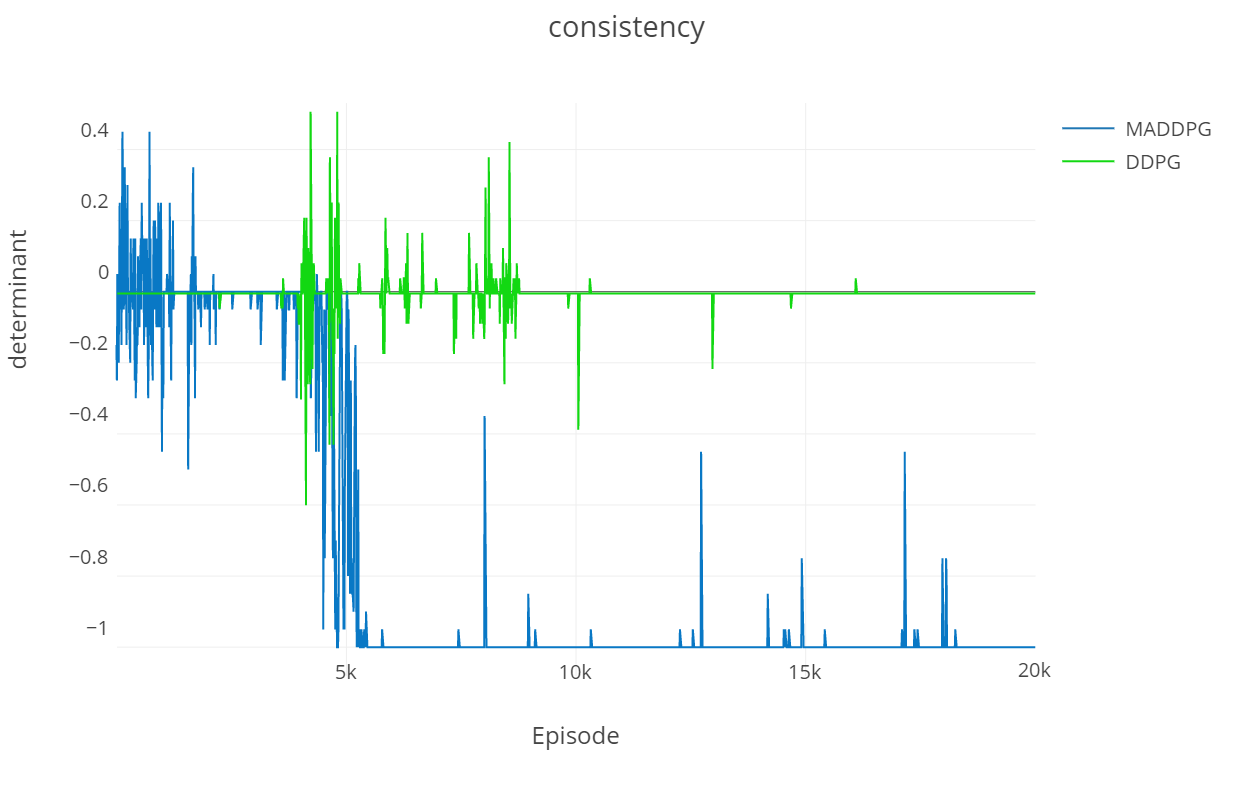
\includegraphics [scale=0.38] {my_folder/images/ch5/ssl-comm.png}
    \caption{График согласованности коммуникаций \textit{говоруна} в сценарии \textit{Simple Speaker Listener}}
    \label{fig:result-ssl-comm}
\end{figure}

Мы построили графики согласованности коммуникаций и вознаграждений для двух агентов в сценарии \textit{Simple Speaker Listener}, которые представлены на \firef{fig:result-ssl-comm} и \firef{fig:result-ssl-rew}. На этих графиках синяя кривая - это результат обучения MADDPG, а зелёная - DDPG.

График на \firef{fig:result-ssl-comm} показывает сходимость консистентности действий общения для \textit{говоруна}, как описано в разделе \hyperref[exp-ssl]{Сценарии}. Этот график показывает, что сходится он только для MADDPG. Это указывает на то, что \textit{говорун}, обученный MADDPG, может постоянно интерпретировать ориентир в одной и той же кодировке, в то время как \textit{говорун}, обученный DDPG, не может поддерживать консистентное общение.

\begin{figure}[ht!]
    \center
    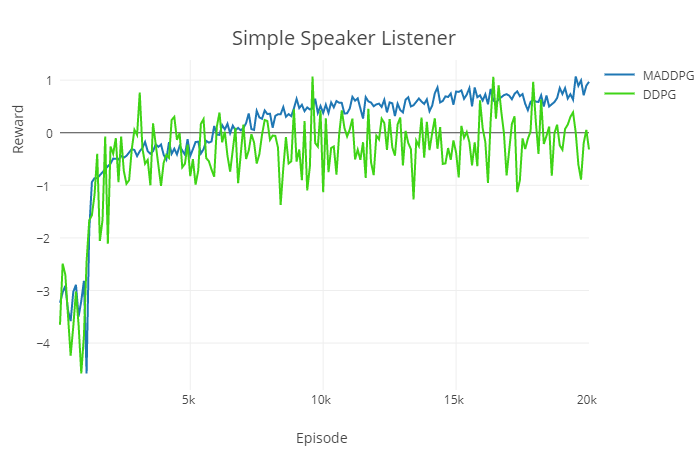
\includegraphics [scale=0.60] {my_folder/images/ch5/ssl-rew.png}
    \caption{График среднего вознаграждения для двух агентов в сценарии Simple Speaker Listener. Результаты обучения по алгоритму MADDPG и DDPG}
    \label{fig:result-ssl-rew}
\end{figure}

График на \firef{fig:result-ssl-rew} показывает среднее вознаграждение, которое агенты получили в конце каждого эпизода. Из этого графика видно, что вознаграждение, полученное агентами, обученными DDPG, ниже, чем агентами, обученными MADDPG.

\begin{figure}[ht!]
    \center
    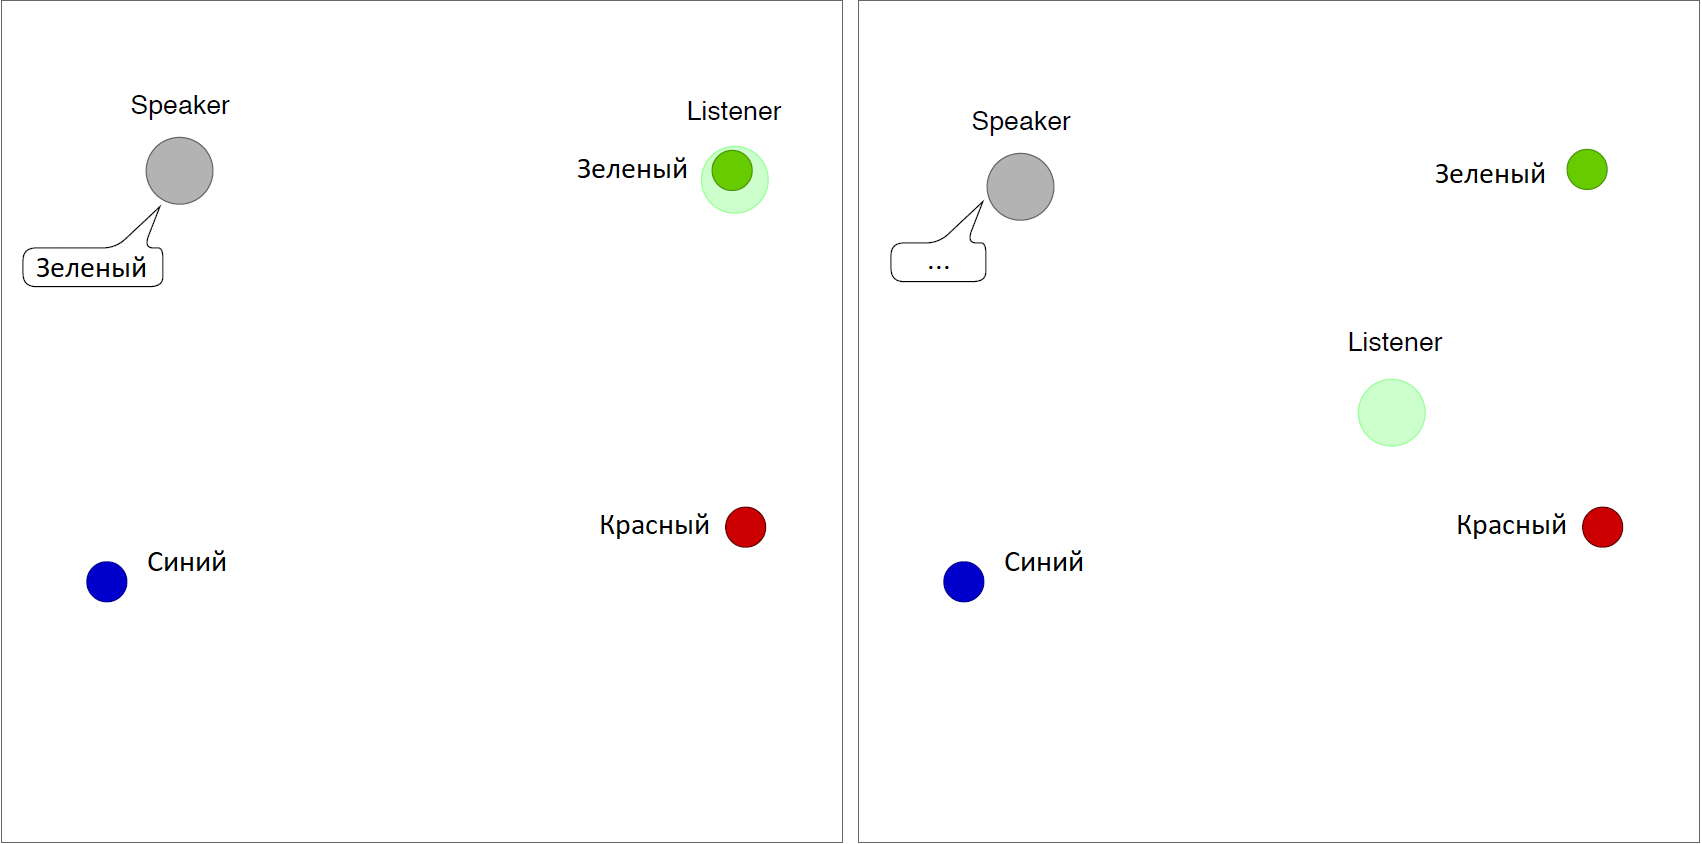
\includegraphics [scale=0.45] {my_folder/images/ch5/results-ssl-conv-non-conv.png}
    \caption{На левой стороне: \textit{говорун} произносит корректное высказывание, \textit{слушатель} перемещается к цели. Справа: коммуникационное действие отсутствует, и \textit{слушатель} застревает между тремя ориентирами (видимо, в попытке минимизировать расстояние до каждого из них)}
    \label{fig:result-conv-non-conv}
\end{figure}

Агенты, обученные DDPG, предпринимают действия, не имея полного наблюдения за состоянием окружающей среды и политикой других агентов. Они не в состоянии изучить политику оптимального взаимодействия друг с другом

На \firef{fig:result-conv-non-conv} показан скриншот при сходимости и не сходимости \textit{Simple Speaker Listener}.

\subsection{Сценарий 2. Simple Reference}

Сценарий \textit{Simple Reference} сходится, когда агенты правильно перемещаются к своим собственным целевым ориентирам. На \firef{fig-intro-sr} показан скриншот поведения агентов после схождения сценария \textit{Simple Reference}. В проведённых экспериментах агенты тренировались алгоритмами DDPG и MADDPG.

\begin{figure}[ht!]
    \center
    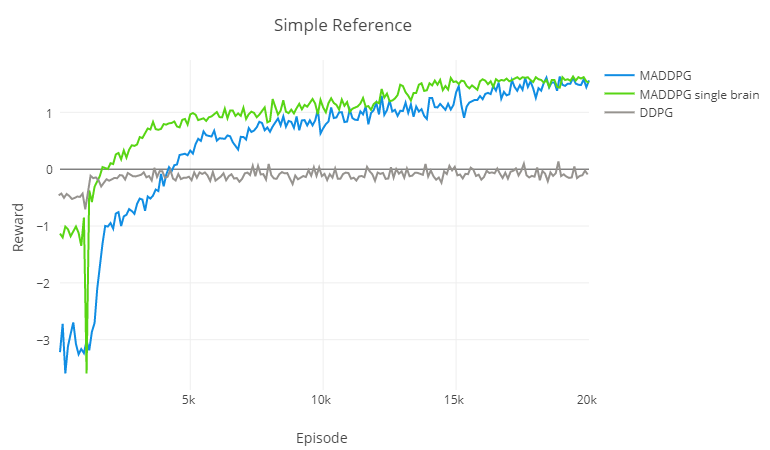
\includegraphics [scale=0.6] {my_folder/images/ch5/sr-rew.png}
    \caption{График среднего вознаграждения для двух агентов в сценарии \textit{Simple Reference}. Результаты обучения по алгоритму MADDPG, MADDPG с одним мозгом и DDPG}
    \label{fig:result-sr-rew}
\end{figure}

\begin{figure}[ht!]
    \center
    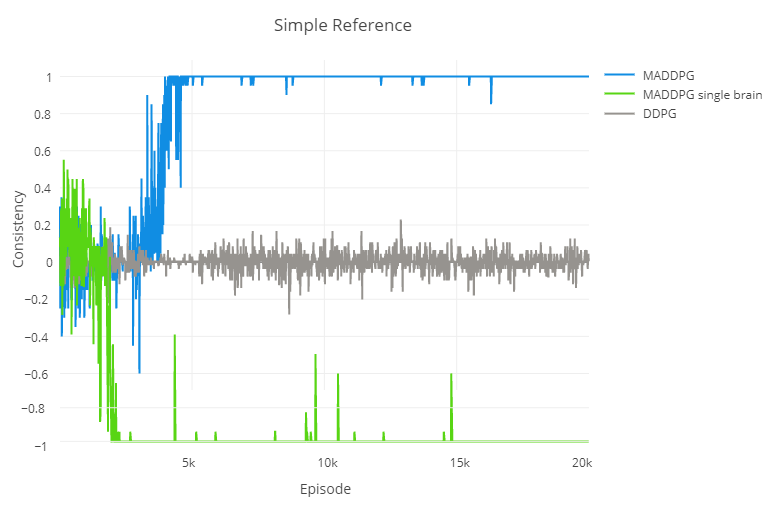
\includegraphics [scale=0.6] {my_folder/images/ch5/sr-comm.png}
    \caption{Графики согласованности взаимодействия для двух агентов в сценарии \textit{Simple Reference}. Результаты обучения по алгоритму MADDPG, MADDPG с одним мозгом и DDPG}
    \label{fig:result-sr-comm}
\end{figure}

Был построен график вознаграждения для двух агентов, который представлен на \firef{fig:result-sr-rew}. На этом графике синяя кривая~--- результат, обученный MADDPG, зелёная~--- одним мозгом, а серая~--- DDPG.

Агенты, обученные с помощью DDPG, получают меньшее вознаграждение, чем агенты MADDPG и его варианты. Также из рендеринга игры видно, что агенты DDPG блуждают среди ориентиров, не зная, какой из них является правильной целью.

Графики на \firef{fig:result-sr-comm} показывают согласованность действий общения. Для MADDPG и его варианта средний детерминант стремится к 1 или -1. Это указывает на то, что агенты, обученные с помощью этих алгоритмов, могут общаться согласованно. Для агентов, обученных DDPG, значение стремится к 0, это иллюстрируют, что они не могут корректно сообщать цели.

В процессе выполнения многочисленных экспериментов можно было наблюдать, что полная несходимость всегда сопровождается тем, что агенты, не способны дифференцировать и сообщать правильные ориентиры друг другу. То же справедливо и для частичной сходимости, когда агенты могут перемещаться только к тем ориентирам, которые правильно сообщены другими агентами, см. \firef{fig:result-sr-non-convergency}. Это также показывает, что агентам для достижения целей необходимо сотрудничать как в физических, так и в коммуникационных действиях.

\begin{figure}[ht!]
    \center
    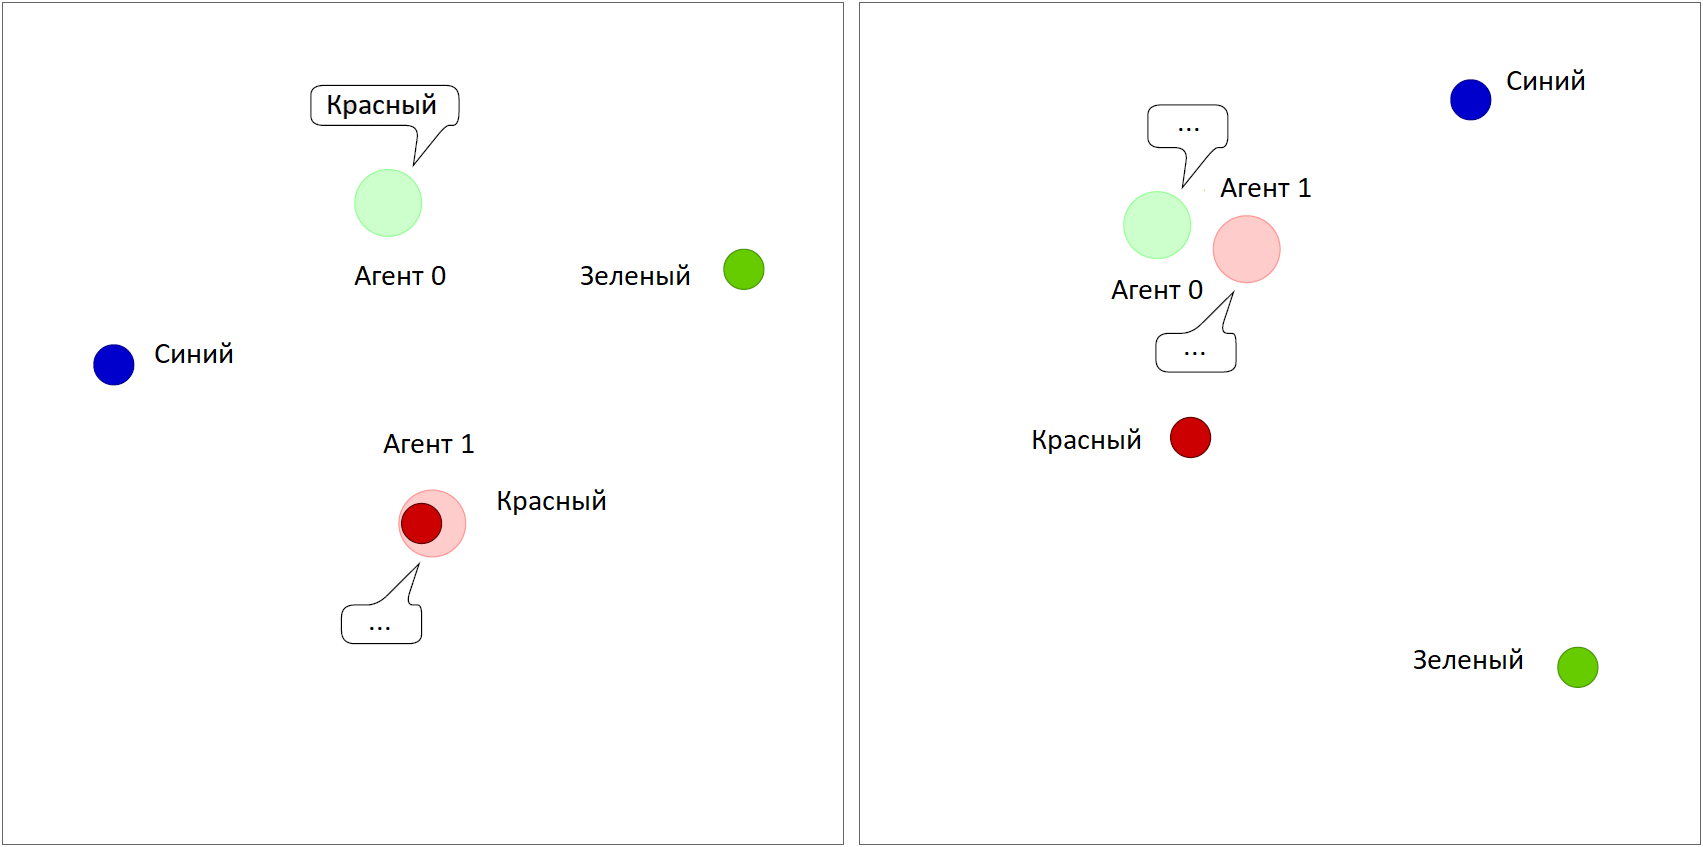
\includegraphics [scale=0.45] {my_folder/images/ch5/results-sr-non-convergency.png}
    \caption{Частичная сходимость с левой стороны: один агент перемещается к цели, а другой ждёт между ориентирами. Несходимость на правой стороне заканчивается тем, что оба агента не знают, куда двигаться и ждут между ориентирами}
    \label{fig:result-sr-non-convergency}
\end{figure}

Наконец, между агентами возникает язык. Проведённые эксперименты показали, что при каждой тренировке агенты по-разному интерпретируют ориентиры. Например, после одной тренировки красный ориентир может выглядеть как ${[1; 0; 0]}$, а после другой~--- как ${[0; 1; 0]}$ или ${[0; 0; 1]}$.

\begin{table}[t!]
    \centering\small
    \caption{Среднее время, потраченное на обучение с различными алгоритмами в 20000 эпизодах}
    \label{tab-sr-time}
    \begin{tabular}{|l|l|l|l|l|l|}
        \hline
        & DDPG           & MADDPG          & MADDPG с одним мозгом \\
        \hline
        Время, 20000 эпизодов & 698 $\pm$ 58~с & 820 $\pm$ 98~с & 635 $\pm$ 45~с       \\ \hline
    \end{tabular}
    \normalsize% возвращаем шрифт к нормальному
\end{table}

В \taref{tab-sr-time} показано время, затраченное на обучение по сценарию \textit{Simple Reference} с разными алгоритмами.

\subsection{Сценарий 3: Simple World Communication}

Мы построили графики вознаграждений и согласованности коммуникаций для двух преследователей и одной жертвы в сценарии \textit{Simple World Communication}, которые представлены на \firef{fig:result-swc-rew} и \firef{fig:result-swc-comm}. На этих графиках зеленая кривая - это результат обучения MADDPG, а серая - DDPG. Все они обучены по 20000 эпизодов.

\begin{figure}[ht!]
	\center
	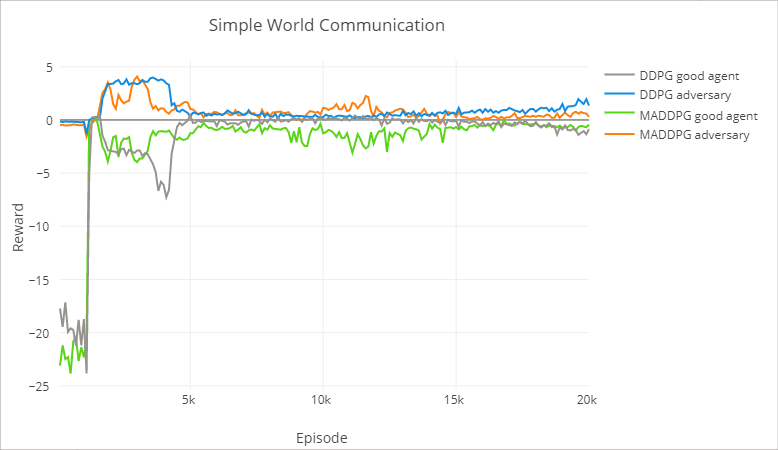
\includegraphics [scale=0.6] {my_folder/images/ch5/swc-rew.png}
	\caption{Среднее вознаграждение преследователей и жертвы с алгоритмами DDPG и MADDPG.}
	\label{fig:result-swc-rew}
\end{figure}

\begin{figure}[ht!]
	\center
	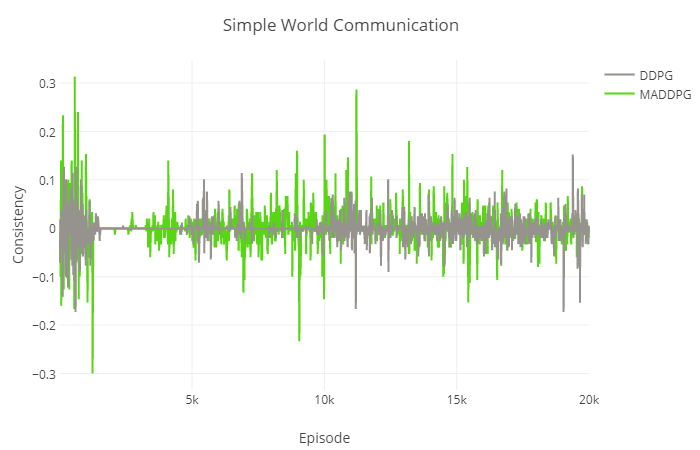
\includegraphics [scale=0.6] {my_folder/images/ch5/swc-comm.png}
	\caption{График консистентности действий коммуникации для алгоритмов DDPG и MADDPG.}
	\label{fig:result-swc-comm}
\end{figure}

К сожалению, из-за ограниченности времени и вычислительных ресурсов, нам не удалось добиться сходимости консистентности действий общения в этом сценарии, это видно на \firef{fig:result-swc-comm}. Из графика видно, что отклонения от нуля больше в случае MADDPG, но этого оказалось недостаточно для того, чтобы «закрепить результат», научиться преследователю использовать получаемые сигналы лидера так, чтобы улучшить общее вознаграждение.

В следствие чего, результаты алгоритма MADDPG ничем не выделяются по сравнению с DDPG, это можно видеть на \firef{fig:result-swc-rew}.

Так же, в этом сценарии трудно установить «конец игры», когда цель достигнута, так как во время обучения агенты обоих команд постепенно действуют все более адекватно, однако это трудно увидеть, на графике среднего вознаграждения. То преследователи изобретают более-менее эффективную тактику, и получают большую награду, то жертва обучается на своих ошибках и начинает учитывать это. Однако, на рендеринге можно видеть, что и преследователи, и жертва ведут себя вполне адекватно. Преследователи догоняют жертву, жертва убегает и, по возможности, стремиться к еде.

Скорее всего, если обучать модель дольше, мы бы увидели более сложные и согласованные действия преследователей.

\subsection{Сценарий 4: Simple Tag}

Как уже упоминалось \hyperref[exp-st]{выше}, этот сценарий не подразумевает коммуникационных действий. Но он был выбран нами, так как он достаточно сложный, и при этом агенты из одной команды имеют одинаковые пространства наблюдения и действий, что позволяет применить вариант алгоритма MADDPG с общим мозгом.

\paragraph{Двое против одного.}

Мы поставили эксперимент с двумя преследователями и одной жертвой.

На \firef{fig-st-reward-ad} и \firef{fig-result-st-reward-ag} изображены графики средней награды преследователей и жертв. Видно, что графики симметричны. Когда преследователи выучиваются двигаться в нужном направлении и понимают, что нужно гонятся за жертвой, они получают большую награду, а жертва меньшую. После чего, жертва выучивается убегать от преследователей - тогда её награда растёт, а награда преследователей снижается. Так же, как и в \hyperref[exp-results-svc]{предыдущем сценарии}.

\begin{figure}[!htbp]
    \adjustbox{minipage=1.3em,valign=t}{\subcaption{}\label{fig-st-reward-ad}}%
    \begin{subfigure}[t]{\dimexpr.5\linewidth-1.3em\relax} %разрешили выделить 0,5 стр в ширину на рисунок
        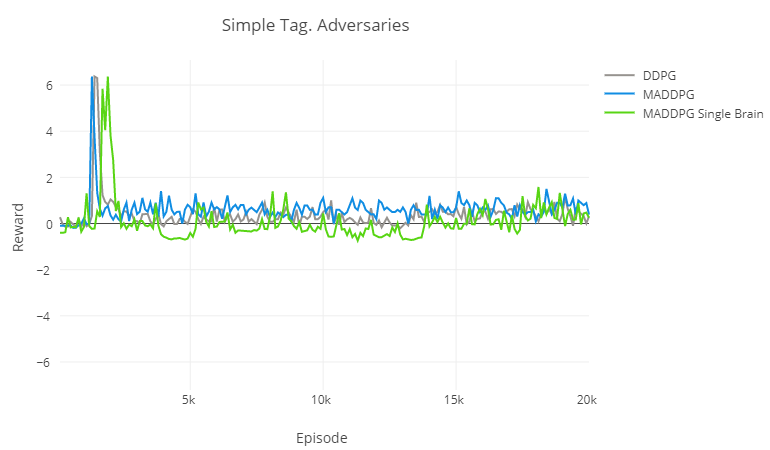
\includegraphics[height=0.19\textheight,valign=t]{my_folder/images/ch5/st-reward-ad.png} %высоту рисунка выставили как 0,3 от высоты наборного поля
    \end{subfigure}
    %	\hfill %выровнять по ширине
    \adjustbox{minipage=1.3em,valign=t}{\subcaption{}\label{fig-result-st-reward-ag}}%
    \begin{subfigure}[t]{\dimexpr.5\linewidth-1.3em\relax}%разрешили выделить 0,5 стр в ширину на рисунок
        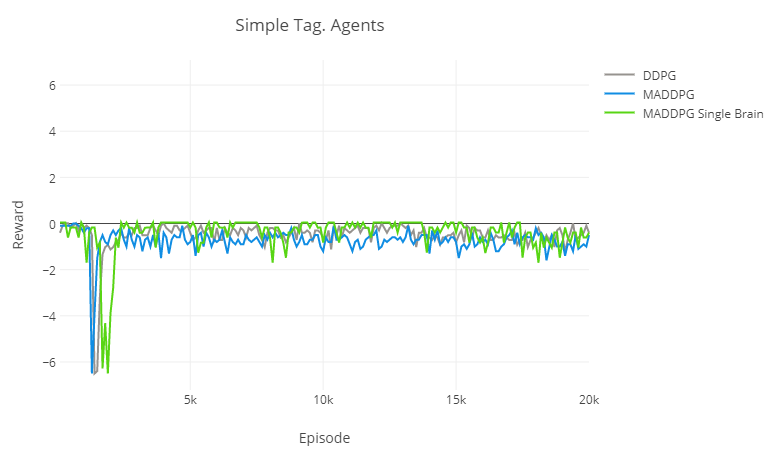
\includegraphics[height=0.19\textheight,valign=t]{my_folder/images/ch5/st-reward-ag.png}%высоту рисунка выставили как 0,3 от высоты наборного поля
    \end{subfigure}
    \captionsetup{justification=centering} %центрировать
    \caption{Награда с применением алгоритма DDPG, MADDPG, MADDPG с общим мозгом: {\itshape a} --- \textit{преследователей}; {\itshape b}~--- \textit{жертв}}\label{fig:spbpu_main_bld-two-photos}
\end{figure}

В \taref{tab-st-time} указано время, затраченное на обучение в данной конфигурации для разных алгоритмов.

\begin{table}[t!]
    \centering\small
    \caption{Среднее время, потраченное на обучение с различными алгоритмами в 20000 эпизодов. 2 преследователя, 1 жертва.}
    \label{tab-st-time}
    \begin{tabular}{|l|l|l|l|l|l|}
        \hline
        & DDPG       & MADDPG      & MADDPG с одним мозгом \\
        \hline
        Время, 20000 эпизодов & 7ч. 46мин. & 10ч. 24мин. & 3ч. 42мин.            \\ \hline
    \end{tabular}
    \normalsize% возвращаем шрифт к нормальному
\end{table}

\paragraph{Четверо против двоих.}

Так же, на этом сценарии мы поставили эксперименты с более сложными настройками - 4 \textit{преследователя} и 2 \textit{жертвы}.

\begin{figure}[!htbp]
    \adjustbox{minipage=1.3em,valign=t}{\subcaption{}\label{fig-result-st-4vs2-ddpg}}%
    \begin{subfigure}[t]{\dimexpr.5\linewidth-1.3em\relax} %разрешили выделить 0,5 стр в ширину на рисунок
        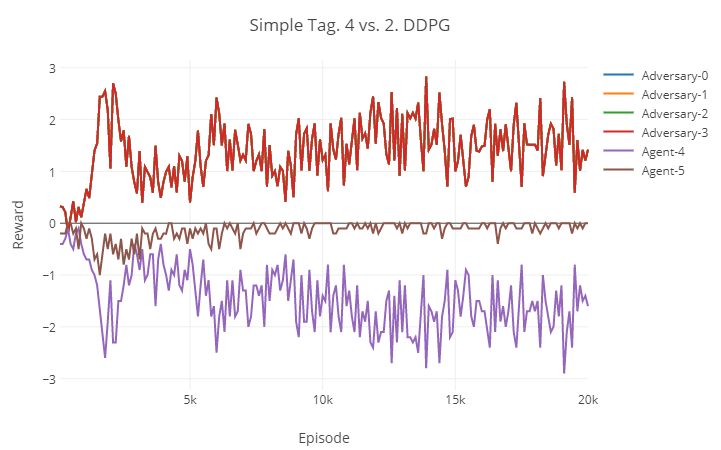
\includegraphics[height=0.20\textheight,valign=t]{my_folder/images/ch5/st-4vs2-ddpg.png} %высоту рисунка выставили как 0,3 от высоты наборного поля
    \end{subfigure}
    %	\hfill %выровнять по ширине
    \adjustbox{minipage=1.3em,valign=t}{\subcaption{}\label{fig-result-st-4vs2-maddpg}}%
    \begin{subfigure}[t]{\dimexpr.5\linewidth-1.3em\relax}%разрешили выделить 0,5 стр в ширину на рисунок
        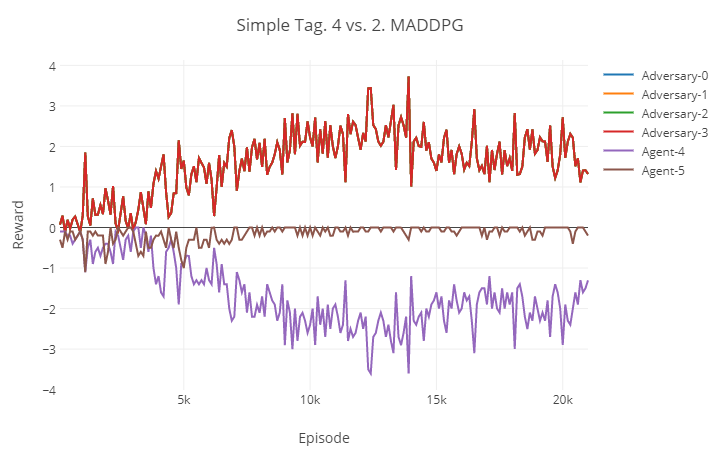
\includegraphics[height=0.20\textheight,valign=t]{my_folder/images/ch5/st-4vs2-maddpg.png}%высоту рисунка выставили как 0,3 от высоты наборного поля
    \end{subfigure}
    \adjustbox{minipage=1.3em,valign=t}{\subcaption{}\label{fig-result-st-4vs2-maddpg-sb}}%
    \begin{subfigure}[t]{\dimexpr.5\linewidth-1.3em\relax}%разрешили выделить 0,5 стр в ширину на рисунок
        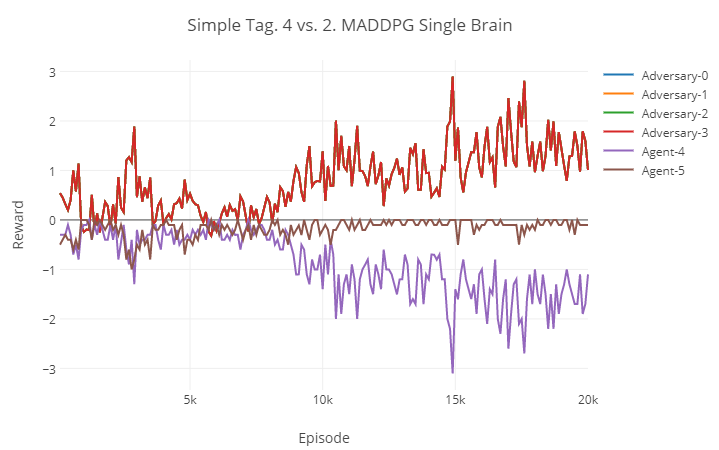
\includegraphics[height=0.20\textheight,valign=t]{my_folder/images/ch5/st-4vs2-maddpg-sb.png}%высоту рисунка выставили как 0,3 от высоты наборного поля
    \end{subfigure}
    \captionsetup{justification=centering} %центрировать
    \caption{Награда каждого из 6 агентов с применением алгоритма: {\itshape a} --- DDPG; {\itshape b}~--- MADDPG; {\itshape c}~--- MADDPG с общим мозгом}\label{fig:spbpu_main_bld-two-photos}
\end{figure}

На \firef{fig-result-st-4vs2-ddpg}, \firef{fig-result-st-4vs2-maddpg} и \firef{fig-result-st-4vs2-maddpg-sb} изображены графики средней награды преследователей и жертв.

В \taref{tab-st-4vs2-time} указано время, затраченное на обучение в данной конфигурации для разных алгоритмов.

\begin{table}[t!]
    \centering\small
    \caption{Среднее время, потраченное на обучение с различными алгоритмами в 20000 эпизодов. 4 преследователя, 2 жертвы.}
    \label{tab-st-4vs2-time}
    \begin{tabular}{|l|l|l|l|l|l|}
        \hline
        & DDPG        & MADDPG      & MADDPG с одним мозгом \\
        \hline
        Время, 20000 эпизодов & 11ч. 23мин. & 16ч. 48мин. & 8ч. 3мин.             \\ \hline
    \end{tabular}
    \normalsize% возвращаем шрифт к нормальному
\end{table}

\paragraph{Вывод из результатов эксперимента.}

Как уже упоминалось выше, награды преследователей и жертв симметрично-противоположны. Это вытекает из того, что: во-первых - сам сценарий имеет конкурентную природу, а награда одним агентам даётся за то же, за что у других отнимается (это описано в разделе \hyperref[intro-st]{Вводная глава: Сценарий 4. Simple Tag}); во-вторых - во время тренировки, обучаются как пресделователи, так и жертвы.

Если взять обученную модель агента одной из команд и начать тренировать против него агантов другой команды, но при этом не обучать первого агента, то мы могли бы увидеть некоторой прогресс, увидеть на графике, как награда первого агента со временем снижается, а его противников - растёт.

Приведённые выше графики наград отчётливо это показывают. В ходе обучения они ни к чему не сходятся.

Однако, это не значит, что агенты не обучаются. При запуске игры на обученных моделях видно, что агенты из обоих команд ведут себя вполне адекватно - преследователи гоняются за жертвами, жертвы избегают преследователей. Как на правом скриншоте на \firef{fig:st}.

И это не помешало нам измерить затраченное время на выполнение каждого эксперимента.

Из таблиц \taref{tab-st-time} и \taref{tab-st-4vs2-time} видно, что алгоритм DDPG показал лучшие результаты, чем MADDPG. Это объясняется тем, что этот алгоритм проще и требует меньших вычислительных мощьностей, в то же время, он не даёт тех возможностей коммуникации, которые могут быть необходимы во многих задачах.

Зато алгоритм MADDPG \textit{с общим мозгом} показал значительное преимущество. Это объясняется тем, что в этом случае не происходит обучения одному и тому же разных наборов сетей актора-критика. Обучается один "мозг" для каждой команды агентов.



\section{Выводы и замечания}

Алгоритм MADDPG считается довольно капризным и требует тонкой настройки. Во время проведения экспериментов алгоритм сходился далеко не всегда, а некоторые эксперименты так и не увенчались успехом.

Обучение сходится с алгоритмом MADDPG, а также с вариантом с \textit{одним мозгом}. К сожалению, при выполнении эксперимента с \textit{учебной программой} не удаётся применить модель, обученную на простых настройках к более сложным. Модель, хорошо выступающая на простом уровне, расходится после повышения уровня сложности. Причиной является то, что при усложнении настроек среды растёт и размерность вектора наблюдений. А также, возможно, то, что обучение модели происходит не сразу, а после наполнения буфера.

Эксперимент с \textit{декомпозированной наградой} тоже не увенчался успехом, вероятно, потому что награда поступает из среды за общее действие, а не за отдельные поддействия. Возможно, если обучать модель значительно дольше, можно было бы увидеть более хорошие результаты.


\newpage
           	 % Глава 3
\ContinueChapterEnd % завершить размещение глав <<подряд>>
%% Завершение основной части

\chapter*{Заключение} \label{ch-conclusion}
\addcontentsline{toc}{chapter}{Заключение}    % в оглавление

Как это было сказано во \hyperref[intro]{введении}, целью данной работы является разработка и исследование алгоритмов управления МАС с применением технологий глубокого обучения с подкреплением. 

Во время работы над этой выпускной работой были решены поставленные задачи: был произведён обзор технологии глубокого обучения с подкреплением, а также методов и алгоритмов управления МАС; были поставлены вопросы исследования, а затем выбраны и доработаны алгоритмы и игровые сценарии, которые позволяют дать ответы на эти вопросы; поставлены эксперименты и сделаны выводы.

В ходе исследования мы пришли к выводу, что лучше всего для управления в основном алгоритм \hyperref[acr:maddpg]{MADDPG}. Сам алгоритм хорошо описан \cite{lowe2017multiagent}. Мы же решили исследовать, могут ли агенты сотрудничать, а также общение агентов между собой. Как упоминалось \hyperref[ch2:ma-algs]{выше}, многие задачи из реального мира лучше решаются многоагентными алгоритмами, для достижения оптимального результата, действия агентов должны быть скоординированы.

С другой стороны, чем больше агентов и чем сложнее среда, тем больше ресурсов требуется на обучение. Поэтому следующий вопрос был посвящён методам оптимизации обучения.

Данная работа способствует дальнейшему пониманию совместной работы множества агентов в игровой среде. Проведённые эксперименты доказывают, что агенты должны вырабатывать оптимальную политику сотрудничества с учётом полного наблюдения за состоянием окружающей среды и политиками других агентов. Очевидно, что в результате обучения возникает композиционный язык, который улучшает сотрудничество. К сожалению, в данной работе алгоритм работает в определённых сценариях, но не удалось реализовать все задуманные приёмы, и не все реализованные варианты алгоритма удалось заставить работать, вероятно, из-за нехватки времени и ресурсов.

По сравнению с предыдущими работами эта дипломная работа расширяет MADDPG до более сложного сценария, когда агентам необходимо сотрудничать в многомерных пространствах действий. Вкратце, агенты одновременно выполняют физическое движение и коммуникационное высказывание.

Некоторые варианты MADDPG исследуются для разных игровых сценариев.

MADDPG с разложенным вознаграждением может быть адаптирован к сценариям со сложным глобальным вознаграждением.

MADDPG с \textit{одним мозгом} может применяться, если агенты в сценарии симметричны в пространстве наблюдения и действий и имеют одинаковое глобальное вознаграждение. Кроме того, агенты, обученные MADDPG с \textit{одним мозгом}, говорят на одном языке, что важно для сценариев, с более чем двумя агентами, которые должны общаться между собой для достижения общей цели.

Как уже упоминалось \hyperref[exp-results-svc]{выше}, из-за конкурентной природы сценариев \textit{Simple World Communication} и \textit{Simple Tag}, нам не удалось добиться того, чтобы награда агентов из разных команд стремилась к какому-то значению или постоянно росла. Мы выбрали эти сценарии для того, чтобы исследовать вопросы поставленные нами в \hyperref[intro-questions]{начале данной работы}.

Зато эксперименты с этими сценариями показали эффективность алгоритма MADDPG \textit{с общим мозгом}.

Опишем возможную \textbf{дальнейшую работу} в продолжение данного исследования.

Алгоритм MADDPG считается довольно капризным и требующим тонкой настройки. Возможно поэтому, а также из-за недостатка времени и вычислительных ресурсов, не увенчались успехом эксперименты по некоторым методам оптимизации обучения: \textit{декомпозированное вознаграждение} и \textit{обучение по учебной программе}.

\textbf{Следующие шаги} в данном исследовании могут быть связаны с тем, чтобы всё-таки реализовать эти методы и поставить соответствующие эксперименты.

Затем следует исследовать сотрудничество большего количества агентов. Они могут обладать более многомерным пространством действий. Агенты должны говорить на одном языке, если необходимо общение между более чем двумя агентами. Следовательно, алгоритмы и сети необходимо модифицировать и адаптировать с учётом новых ситуаций. Приведённые выше выводы в этой дипломной работе могут способствовать дальнейшим исследованиям.

Следующее усложнение - это использование алгоритма \hyperref[acr:dpg]{детерминированного градиента политики} для задач с несколькими агентами в сценариях трёхмерных игр. Основной проблемой для алгоритма в сценариях 3D-игр может быть высокоразмерный ввод пикселей. Дальнейшая работа должна быть сделана соответственно над структурой нейронных сетей, например, сверточных слоёв в \textit{акторе} и настройке гиперпараметров.

Все эти этапы - это шаги с постепенным усложнением задач, перед попыткой применения уже отработанных алгоритмов к управлению роботами и их совместной командной работе.

Основные сложности применения алгоритмов \hyperref[acr:rl]{обучения с подкреплением} к управлению роботами, заключаются в:
\begin{itemize}
	\item очень высокая размерность наблюдения;
	\item высокая степень неопределённости (мы никогда до конца не знаем, как поменяется среда после очередного нашего действия);
	\item очень тренировать модель в реальной среде очень дорого, долго (мы не можем ускорить течение времени за счёт вычислительных мощностей), а часто и вовсе невозможно, поскольку в процессе обучения неизбежны ошибки, и, например автомобиль, управляемый программой, может представлять опасность.
\end{itemize}

Мы считаем, что из всего вышесказанного следует, что первые этапы изучения следует производить в симуляторах естественной среды.

И наконец, следующим шагом было бы пробовать применить алгоритм к обучению нескольких роботов для достижения общей цели в реальной среде. Например, сбор мусора, различные задачи на преследование и т. д.

Напоследок, хотелось бы выразить бладодарность за помощь в написании данной работы моему научному руководителю, доценту ВШиСТ - Паку Вадиму Геннадьевичу, а так же научному сотруднику СПИИРАН - Клеверову Денису Анатольевичу, за помощь в технических вопросах и за рецензию. Без вас этой работы не было бы.
        	 % Заключение

%% Наличие следующих перечней не исключает расшифровку сокращения и условного обозначения при первом упоминании в тексте!
\chapter*{Список сокращений и условных обозначений}             % Заголовок
\addcontentsline{toc}{chapter}{Список сокращений и условных обозначений}  % Добавляем его в оглавление
\noindent
\addtocounter{table}{-1}% Нужно откатить на единицу счетчик номеров таблиц, так как следующая таблица сделана для удобства представления информации по ГОСТ
%\begin{longtabu} to \dimexpr \textwidth-5\tabcolsep {r X}
\begin{longtabu} to \textwidth {r X} % Таблицу не прорисовываем!
% Жирное начертание для математических символов может иметь
% дополнительный смысл, поэтому они приводятся как в тексте
% диссертации
\textbf{МАС}  & Мультиагентная система. \label{acr:mas} \\
\textbf{ML}  & Машинное обучение (Machine Learning). \label{acr:ml} \\
\textbf{DL}  & Глубокое обучение (Deep Learning). \label{acr:dl} \\
\textbf{RL}  & Обучение с подкреплением (Reinforcement Learning). \label{acr:rl} \\
\textbf{DRL}  & Глубокое обучение с подкреплением (Deep Reinforcement Learning). \label{acr:drl} \\
\textbf{DPG}  & Детерминированный градиент политики (Deterministic Policy Gradient). \label{acr:dpg} \\
\textbf{DDPG}  & Глубокий детерминированный градиент политики (Deep Deterministic Policy Gradient). \label{acr:ddpg} \\
\textbf{MADDPG}  & Мультиагентный глубокий детерминированный градиент политики (Multiagent Deep Deterministic Policy Gradient). \label{acr:maddpg} \\
\textbf{COMA}  & Контрафактный мультиагентный градиент политики (Counterfactual Multi-Agent Policy Gradient, COMA). \label{acr:coma} \\
\textbf{ИНС}  & Искусственная нейронная сеть (Artificial Neural Network). \label{acr:ann} \\
\textbf{МППР}  & Марковский процесс принятия решений (Markov Decision Process, MDP). \label{acr:mdp} \\
%$\begin{rcases}
%a_n\\
%b_n
%\end{rcases}$  & 
%\begin{minipage}{\linewidth}
%Коэффициенты разложения Ми в дальнем поле, соответствующие
%электрическим и магнитным мультиполям.
%\end{minipage}
%\\
%${\boldsymbol{\hat{\mathrm e}}}$ & Единичный вектор. \\
%$E_0$ & Амплитуда падающего поля.\\
%$\begin{rcases}
%a_n\\
%b_n
%\end{rcases}$  & 
%Коэффициенты разложения Ми в дальнем поле соответствующие
%электрическим и магнитным мультиполям ещё раз, но без окружения
%minipage нет вертикального выравнивания по центру.
%\\
%$j$ & Тип функции Бесселя.\\
%$k$ & Волновой вектор падающей волны.\\
%
%$\begin{rcases}
%a_n\\
%b_n
%\end{rcases}$  & 
%\begin{minipage}{\linewidth}
%\vspace{0.7em}
%Коэффициенты разложения Ми в дальнем поле соответствующие
%электрическим и магнитным мультиполям, теперь окружение minipage есть
%и добавленно много текста, так что описание группы условных
%обозначений значительно превысило высоту этой группы... Для отбивки
%пришлось добавить дополнительные отступы.
%\vspace{0.5em}
%\end{minipage}
%\\
%$L$ & Общее число слоёв.\\
%$l$ & Номер слоя внутри стратифицированной сферы.\\
%$\lambda$ & Длина волны электромагнитного излучения
%в вакууме.\\
%$n$ & Порядок мультиполя.\\
%$\begin{rcases}
%{\mathbf{N}}_{e1n}^{(j)}&{\mathbf{N}}_{o1n}^{(j)}\\
%{\mathbf{M}_{o1n}^{(j)}}&{\mathbf{M}_{e1n}^{(j)}}
%\end{rcases}$  & Сферические векторные гармоники.\\
%$\mu$  & Магнитная проницаемость в вакууме.\\
%$r,\theta,\phi$ & Полярные координаты.\\
%$\omega$ & Частота падающей волны.\\
%
%  \textbf{BEM} & Boundary element method, метод граничных элементов.\\
%  \textbf{CST MWS} & Computer Simulation Technology Microwave Studio.
\end{longtabu}
		         % Необязательная рубрика! Список сокращений и условных обозначений

\input{my_folder/dictionary}    		 % Необязательная рубрика! Словарь терминов
% По порядку после Списка сокращений и условных обозначений, если есть.


\input{my_folder/references}		     % Список литературы

% Здесь можно поместить список иллюстративного материала

\appendix % не редактировать / keep unmodified


%\chapter{Краткие инструкции по настройке издательской системы \LaTeX}\label{appendix-MikTeX-TexStudio}							% Заголовок
%\addcontentsline{toc}{chapter}{Second call for chapters to participate in the book Machine learning in analysis of biomedical and socio-economic data}	% Добавляем его в оглавление

В SPbPU-BCI-template {\itshape автоматически выставляются необходимые настройки и в исходном тексте шаблона приведены примеры оформления текстово-графических объектов}, поэтому авторам достаточно заполнить имеющийся шаблон текстом главы (статьи), не вдаваясь в детали оформления, описанные далее. Возможный <<быстрый старт>> оформления главы (статьи) под Windows следующий\footnote{Внимание! Пример оформления подстрочной ссылки (сноски).}:

\begin{enumerate}
	\item Установка полной версии MikTeX  \cite{latex-miktex}.  В процессе установки лучше выставить параметр доустановки пакетов <<на лету>>.
	
	\item Установка TexStudio \cite{latex-texstudio}.
	
%		\item установка шрифтов PSCyr для работы с TimesNew\-Roman\-PSMT  	\href{https://github.com/AndreyAkinshin/Russian-Phd-LaTeX-Dissertation-Template/blob/master/PSCyr/Windows.md}{по данной инструкции}. В итоговом документе будет, скорее всего, использован Newton.
	
%	\item Переименование следующих файлов, где вместо \texttt{AuthorsSur\-names} необходимо подставить фамилии авторов (можно сокращать до первых четырех букв): 
%	
%	\begin{enumerate}
%		\item Основной файл \texttt{Book\_title\_ch\_Authors\-Sur\-names.tex}.
%		\item Библиография \texttt{biblio\textbackslash{}Book\_title\_bib\_Authors\-Sur\-na\-mes\-.bib}.
%		\item Пользовательские настройки (при необходимости), \texttt{common\textbackslash{}Book\_\-tit\-le\_ext\_Authors\-Sur\-names.tex}. 
%	\end{enumerate}
%	
%	\item После открытия основного файла \texttt{Book\_title\_ch\_Authors\-Sur\-names.tex} (с новым названием)   переименовать названия по аналогии в следующих командах \texttt{\textbackslash{}input\{\}}:
%	
%	\begin{enumerate}
%		\item \texttt{biblio/Book\_title\_bib\_Authors\-Sur\-names.bib},
%		\item \texttt{common/Book\_title\_ext\_Authors\-Sur\-names.tex (при необходимости) }.
%	\end{enumerate}
%	
	
	\item Запуск TexStudio и компиляция \verb|my_chapter.tex| с помощью команды <<Build\&View>> (например, с помощью двойной зелёной стрелки в верхней панели). {\itshape Иногда, для достижения нужного результата необходимо несколько раз скомпилировать документ.}
	
	\item В случае, если не отобразилась библиография, можно
	
	\begin{itemize}
		\item воспользоваться командой Tools $\to$ Commands $\to$ Biber, затем запустив Build\&View;
		
		\item настроить автоматическое включение библиографии в настройках Options $\to$ Configure TexStudio $\to$ Build $\to$  Build\&View (оставить по умолчанию, если сборка происходит слишком долго): \texttt{txs:///pdflatex | txs:///biber | txs:///pdflatex | txs:///pdflatex | txs:///\-view-pdf}.
	\end{itemize}
	
\end{enumerate}

В случае возникновения ошибок, попробуйте скомпилировать документ до последних действий или внимательно ознакомьтесь с описанием проблемы в log-файле. Бывает полезным переход (по подсказке TexStudio) в нужную строку в pdf-файле или запрос с текстом ошибке в поисковиках. Наиболее вероятной проблемой при первой компиляции может быть отсутствие какого-либо установленного пакета \LaTeX. 

В случае корректной работы настройки <<установка на лету>> все дополнительные пакеты будут скачиваться и устанавливаться в автоматическом режиме. Если доустановка пакетов осуществляется медленно (несколько пакетов за один запуск компилятора), то можно попробовать установить их в ручном режиме следующим образом:

\begin{enumerate}[1.]
	\item Запустите программу: меню $\to$ все программы $\to$ MikTeX $\to$ Maintenance (Admin) $\to$ MiKTeX Package Manager (Admin).
	\item Пользуясь поиском, убедитесь, что нужный пакет присутствует, но не установлен (если пакет отсутствует воспользуйтесь сначала MiKTeX Update (Admin)).
	\item Выделив строку с пакетом (возможно выбрать несколько или вообще все неустановленные пакеты), выполните установку Tools $\to$ Install или с помощью контекстного меню.
	\item После завершения установки запустите программу MiKTeX Settings (Admin).
	\item Обновите базу данных имен файлов Refresh FNDB.
\end{enumerate}


Для проверки текста статьи на русском языке полезно также воспользоваться настройками Options $\to$ Configure TexStudio $\to$ Language Checking $\to$  Default Language. Если русский язык <<ru\_RU>> не будет доступен в меню выбора, то необходимо вначале выполнить Import Dictionary, скачав из интернета любой русскоязычный словарь. 


%\chapter{\normalfont\normalsize{}Часто задаваемые вопросы (FAQ)}\label{Appendix-FAQ}							% Заголовок
%%\addcontentsline{toc}{chapter}{Second call for chapters to participate in the book Machine learning in analysis of biomedical and socio-economic data}	% Добавляем его в оглавление


Далее приведены формулы \eqref{eq:Pi-app2}, \eqref{eq:Pi-app2-},  \firef{fig:spbpu_hydrotower-app2}, \firef{fig:spbpu_hydrotower-app2-}, \taref{tab:ToyCompare-app2}, \taref{tab:ToyCompare-app2-}.


\begin{equation}% лучше не оставлять пропущенную строку (\par) перед окружениями для избежания лишних отсупов в pdf
\label{eq:Pi-app2-} % eq - equations, далее название, ch поставлено для избежания дублирования
\pi \approx 3,141.
\end{equation}

%
\begin{figure}[ht!] 
	\center
	\includegraphics [scale=0.27] {my_folder/images//spbpu_hydrotower}
	\caption{Вид на гидробашню СПбПУ \cite{spbpu-gallery}} 
	\label{fig:spbpu_hydrotower-app2-}  
\end{figure}

\begin{table} [htbp]% Пример оформления таблицы
	\centering\small
	\caption{Представление данных для сквозного примера по ВКР \cite{Peskov2004}}%
	\label{tab:ToyCompare-app2-}		
	\begin{tabular}{|l|l|l|l|l|l|}
		\hline
		$G$&$m_1$&$m_2$&$m_3$&$m_4$&$K$\\
		\hline
		$g_1$&0&1&1&0&1\\ \hline
		$g_2$&1&2&0&1&1\\ \hline
		$g_3$&0&1&0&1&1\\ \hline
		$g_4$&1&2&1&0&2\\ \hline
		$g_5$&1&1&0&1&2\\ \hline
		$g_6$&1&1&1&2&2\\ \hline		
	\end{tabular}	
	\normalsize% возвращаем шрифт к нормальному
\end{table}




\section{Параграф приложения}\label{app-2-1}							


\subsection{Название подпараграфа} \label{ch2:subsec-title-abbr} %название по-русски


Название параграфа оформляется с помощью команды  \texttt{\textbackslash{}subsection\{...\}}.


\subsubsection{Название подподпараграфа}\label{ch2:subsubsec-title-abbr} %название по-русски

\begin{equation}% лучше не оставлять пропущенную строку (\par) перед окружениями для избежания лишних отсупов в pdf
\label{eq:Pi-app2} % eq - equations, далее название, ch поставлено для избежания дублирования
\pi \approx 3,141.
\end{equation}
%
%
\begin{figure}[ht!] 
	\center
	\includegraphics [scale=0.27] {my_folder/images//spbpu_hydrotower}
	\caption{Вид на гидробашню СПбПУ \cite{spbpu-gallery}} 
	\label{fig:spbpu_hydrotower-app2}  
\end{figure}
%




\begin{table}[t!]% Пример оформления таблицы
	\centering\small
	\caption{Представление данных для сквозного примера по ВКР \cite{Peskov2004}}%
	\label{tab:ToyCompare-app2}		
	\begin{tabular}{|l|l|l|l|l|l|}
		\hline
		$G$&$m_1$&$m_2$&$m_3$&$m_4$&$K$\\
		\hline
		$g_1$&0&1&1&0&1\\ \hline
		$g_2$&1&2&0&1&1\\ \hline
		$g_3$&0&1&0&1&1\\ \hline
		$g_4$&1&2&1&0&2\\ \hline
		$g_5$&1&1&0&1&2\\ \hline
		$g_6$&1&1&1&2&2\\ \hline		
	\end{tabular}	
	\normalsize% возвращаем шрифт к нормальному
\end{table}


%% В случае, когда таблица (рисунок) размещаются на последней странице, для переноса названия приложения на новую строку используем:
\NewPage % начать новое приложение с новой страницы 			     % Приложение 1

%\chapter{Некоторые дополнительные примеры}\label{appendix-extra-examples}							% 

В приложении\footnote{Внимание! Пример оформления подстрочной ссылки (сноски).} приведены формулы \eqref{eq:Pi-app}, \eqref{eq:Pi-app-}, \firef{fig:spbpu_hydrotower-app}, \firef{fig:spbpu_hydrotower-app-}, \taref{tab:ToyCompare-app}, \taref{tab:ToyCompare-app-}


\begin{equation}% лучше не оставлять пропущенную строку (\par) перед окружениями для избежания лишних отсупов в pdf
\label{eq:Pi-app-} % eq - equations, далее название, ch поставлено для избежания дублирования
\pi \approx 3,141.
\end{equation}
%
%
\begin{figure}[ht!] 
	\center
	\includegraphics [scale=0.27] {my_folder/images//spbpu_hydrotower}
	\caption{Вид на гидробашню СПбПУ \cite{spbpu-gallery}} 
	\label{fig:spbpu_hydrotower-app-}  
\end{figure}

\begin{table} [htbp]% Пример оформления таблицы
	\centering\small
	\caption{Представление данных для сквозного примера по ВКР \cite{Peskov2004}}%
	\label{tab:ToyCompare-app-}		
	\begin{tabular}{|l|l|l|l|l|l|}
		\hline
		$G$&$m_1$&$m_2$&$m_3$&$m_4$&$K$\\
		\hline
		$g_1$&0&1&1&0&1\\ \hline
		$g_2$&1&2&0&1&1\\ \hline
		$g_3$&0&1&0&1&1\\ \hline
		$g_4$&1&2&1&0&2\\ \hline
		$g_5$&1&1&0&1&2\\ \hline
		$g_6$&1&1&1&2&2\\ \hline		
	\end{tabular}	
	\normalsize% возвращаем шрифт к нормальному
\end{table}




\section{Подраздел приложения}\label{app-2-1}							


\begin{equation}% лучше не оставлять пропущенную строку (\par) перед окружениями для избежания лишних отсупов в pdf
\label{eq:Pi-app} % eq - equations, далее название, ch поставлено для избежания дублирования
\pi \approx 3,141.
\end{equation}
%
%
\begin{figure}[ht!] 
	\center
	\includegraphics [scale=0.27] {my_folder/images//spbpu_hydrotower}
	\caption{Вид на гидробашню СПбПУ \cite{spbpu-gallery}} 
	\label{fig:spbpu_hydrotower-app}  
\end{figure}

\begin{table} [htbp]% Пример оформления таблицы
	\centering\small
	\caption{Представление данных для сквозного примера по ВКР \cite{Peskov2004}}%
	\label{tab:ToyCompare-app}		
	\begin{tabular}{|l|l|l|l|l|l|}
		\hline
		$G$&$m_1$&$m_2$&$m_3$&$m_4$&$K$\\
		\hline
		$g_1$&0&1&1&0&1\\ \hline
		$g_2$&1&2&0&1&1\\ \hline
		$g_3$&0&1&0&1&1\\ \hline
		$g_4$&1&2&1&0&2\\ \hline
		$g_5$&1&1&0&1&2\\ \hline
		$g_6$&1&1&1&2&2\\ \hline		
	\end{tabular}	
	\normalsize% возвращаем шрифт к нормальному
\end{table}

			 	 % Приложение 2


\end{document} % конец документа


%%% Удачной защиты ВКР! - Good luck on the thesis defense!
%%
%%% Поддержать проект
%%
%% Запросы на добавление / изменение просим писать на следующей странице:
%% https://github.com/ParkhomenkoV/SPbPU-student-thesis-template/issues
%%
%% Список пожеланий в файле шаблона <<TO-DO-list.tex>>
%%
%% Благодарности просим указывать в виде 
%%
%% 1. Добавление <<Звезды>> проекту https://github.com/ParkhomenkoV/SPbPU-student-thesis-template/stargazers
%%
%% 2. Добавления <<Сердечка>> и репоста проекта в социальных сетях:
%%		https://vk.com/latex_polytech 
%%		https://www.fb.com/groups/latex.polytech
%%

%%% Support project
%%
%% Requests on adding / modifications is better to be publishen on the following web-page:
%% https://github.com/ParkhomenkoV/SPbPU-student-thesis-template/issues
%%
%% Wishlist is in the template's file called <<TO-DO-list.tex>>
%%
%% Acknowledgements are better to be done in the form of 
%%
%% 1. Adding <<Star>> to the project https://github.com/ParkhomenkoV/SPbPU-student-thesis-template/stargazers
%%
%% 2. Adding <<Likes>> and Project repost in the social networks:
%%		https://vk.com/latex_polytech 
%%		https://www.fb.com/groups/latex.polytech
%% 

% Check list при передаче ВКР:
% - Количество страниц в Задании 2. Если нет, то комментирование последней строки в my_task.tex
% - Зачистка всех вспомогательных файлов (Clear auxilary files) и компиляция ВКР не менее 3х раз